\documentclass[openany]{book}
\usepackage{titling}
\usepackage{wrapfig}
\usepackage{etoolbox}
\BeforeBeginEnvironment{wrapfigure}{\leavevmode}
\usepackage[utf8]{vietnam}
\usepackage{titlesec}
\usepackage{graphicx}
\usepackage{booktabs}
\usepackage{parskip}
\usepackage{framed}
\usepackage{float}
\usepackage{caption}
\usepackage[protrusion=false,expansion=false]{microtype}
\usepackage{ragged2e}
\usepackage{caption}
\usepackage{multicol}
\usepackage[table]{xcolor}
\usepackage{array}
\usepackage{xurl}
\usepackage[colorlinks=true, urlcolor=blue, linkcolor=black, citecolor=blue]{hyperref}
\usepackage{longtable}
\usepackage{tabularx}
\usepackage{mdframed}
\usepackage{tcolorbox}
\usepackage[utf8]{inputenc}
\usepackage{CJKutf8}
\usepackage[super,square]{natbib}
\makeatletter
\renewcommand\mainmatter{%
    \clearpage
  \@mainmattertrue
  \pagenumbering{arabic}}

\AtBeginDocument{
    \renewcommand{\bibname}{References}
    \renewcommand{\chaptername}{Chapter}
    \renewcommand{\contentsname}{Table of contents}
    }
\setlength\parskip{1em plus 2pt}
\setlength{\droptitle}{-8ex}
% \setlength{\intextsep}{0pt}
\titleformat{\section}
  {\normalfont\Large\bfseries}{\thesection}{0.5em}{\vspace{-9pt}}[{\vspace{-10pt}\rule{0.5\textwidth}{0.8pt}}]

\title{Economy of Vietnam\\ \normalsize Typography of Technical Documents}
\author{Huỳnh Trung Tín-524k00033}
\date{10/09/2025}

\begin{document}
\frontmatter
\maketitle
\chapter*{Dedication}
I would like to dedicate this small segment to my lecturer Nguyễn Quốc Bình, as a thank for you for teaching us how to use Latex and for being patient with us through and through. If you do take your time to read this segment, I just want to say that I appreciate the kindness you have shown us and I hope with your teaching that I, along with many students you have taught, will not fail you.

Sincerely, Huỳnh Trung Tín
\clearpage
\chapter*{Preface}
This report is the cumulation of knowledge gained from previous assignments, along with the use of bibliography. The report aims to refine the previous book format of Economy of Vietnam by adding references and presenting it as a professional academic level Latex book.
\tableofcontents
\mainmatter
\chapter{Economy of Vietnam}

\begin{wrapfigure}{r}{.55\textwidth}
    \vspace{-40pt}
    \caption*{\textbf{Economy of Vietnam}}
    \begin{tcolorbox}[bottomrule=0pt]
        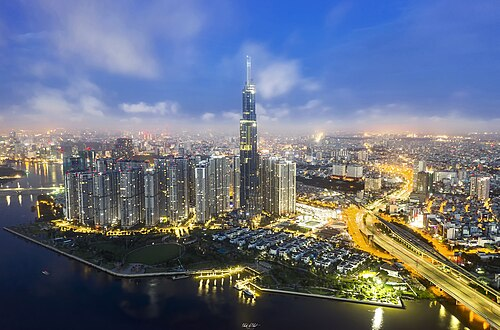
\includegraphics[width=55mm,scale=0.5]{Ho_Chi_Minh_City_-_DJI_0124-HDR.jpg}
        \caption*{\small \centering \href{https://en.wikipedia.org/wiki/Ho_Chi_Minh_City}{Ho Chi Minh City}, the economic capital of Vietnam}
        \small
        \setlength{\tabcolsep}{4pt}
        \begin{tabularx}{\linewidth}{@{} >{\raggedright\arraybackslash}p{2.5cm} >{\raggedright\arraybackslash}X@{}}

            \textbf{Currency}            & {Vietnamese đồng (VND; ₫)}                                                                                                                                                    \\
            {\textbf{Fiscal year}}       & {Calendar year}                                                                                                                                                               \\
            \textbf{Trade organisations} & {AFTA, WTO, APEC, ASEAN, RCEP, CPTPP, FAO}                                                                                                                                    \\
            \\
            \textbf{Country group}       & { \begin{tabular}[l]{@{}p{2.8cm}@{}}\raggedright Developing/\newline Emerging\\ Lower-middle income\newline country\\ Socialist-oriented\newline market economy\end{tabular}} \\
        \end{tabularx}
    \end{tcolorbox}
\end{wrapfigure}


\begin{sloppypar}\RaggedRight
The economy of Vietnam is a \href{https://en.wikipedia.org/wiki/Developing_economy}{developing} \href{https://en.wikipedia.org/wiki/Mixed_economy}{mixed} \href{https://en.wikipedia.org/wiki/Socialist-oriented_market_economy}{socialist-oriented market economy}\cite{3}. It is the \href{https://en.wikipedia.org/wiki/List_of_countries_by_GDP_(nominal)}{33rd-largest economy} in the world by \href{https://en.wikipedia.org/wiki/Nominal_gross_domestic_product}{nominal gross domestic product} (GDP) and the \href{https://en.wikipedia.org/wiki/List_of_countries_by_GDP_(PPP)}{26th-largest economy} in the world by \href{https://en.wikipedia.org/wiki/Purchasing_power_parity}{purchasing power parity} (PPP). It is an upper-middle income country with a low cost of living. \href{https://en.wikipedia.org/wiki/Vietnam}{Vietnam} is a member of the \href{https://en.wikipedia.org/wiki/Asia-Pacific_Economic_Cooperation}{Asia-Pacific Economic Cooperation}, the \href{https://en.wikipedia.org/wiki/Association_of_Southeast_Asian_Nations}{Association of Southeast Asian Nations} and the \href{https://en.wikipedia.org/wiki/World_Trade_Organization}{World Trade Organization}.
\end{sloppypar}



\begin{sloppypar}
    Since the mid-1980s, through the
    \href{https://en.wikipedia.org/wiki/%C4%90%E1%BB%95i_M%E1%BB%9Bi}{Đổi Mới} reform period, Vietnam has made a shift from a 
    \href{https://en.wikipedia.org/wiki/Centralization}{highly centralized}
    \href{https://en.wikipedia.org/wiki/Planned_economy}{planned economy} to a
    \href{https://en.wikipedia.org/wiki/Mixed_economy}{mixed economy}.

    Before, \href{https://en.wikipedia.org/wiki/North_Vietnam}{South Vietnam} was reliant on U.S. aid,\cite{26}
    while North Vietnam and reunified Vietnam relied on communist aid until the
    \href{https://en.wikipedia.org/wiki/Dissolution_of_the_Soviet_Union}{Soviet Union's dissolution}.\cite{27}
\end{sloppypar}

\clearpage
\begin{wrapfigure}{r}{.55\textwidth}
    \begin{tcolorbox}[toprule=0pt , bottomrule=0pt]
        \small
        \setlength{\tabcolsep}{4pt}
        \begin{tabularx}{\linewidth}{@{}>{\raggedright\arraybackslash}p{2.8cm} >{\raggedright\arraybackslash}X@{}}
            \multicolumn{2}{@{}>{\centering\arraybackslash}p{\dimexpr\linewidth\relax}@{}}{\cellcolor[HTML]{ADD8E6}\textbf{Statistics}}                                                                    \\
            \textbf{Population}                     & 101,598,527 (2025)                                                                                                                                   \\
            \\
            {\textbf{GDP}}                          & \begin{tabular}[c]{@{}>{\raggedright\arraybackslash}p{2.5cm}@{}} \$490.97 billion (nominal; 2025)\\ \$1.762 trillion (PPP; 2025)\end{tabular}        \\
            \\
            \textbf{GDP rank}                       & {\begin{tabular}[c]{@{}>{\raggedright\arraybackslash}p{2.5cm}@{}}33rd (nominal; 2025)\\ 23rd (PPP; 2025)\end{tabular}}                               \\
            \textbf{GDP growth}                     & \begin{tabular}[c]{@{}>{\raggedright\arraybackslash}p{2.5cm}@{}} 7.09\% (2024)\\  5.8\% (2025)\\ 4\% (2026)\end{tabular}                               \\
            \textbf{GDP per capita}                 & \begin{tabular}[c]{@{}>{\raggedright\arraybackslash}p{2.5cm}@{}}\$4,806 (nominal; 2\-0\-2\-5 e\-s\-t.)\\\$17,484 (PPP; 2025 est.)\end{tabular}        \\
            \\
            \textbf{GDP per capita rank}            & {\begin{tabular}[c]{@{}>{\raggedright\arraybackslash}p{2.5cm}@{}}119th (nominal; 2025)\\ 104th (PPP; 2025)\end{tabular}}                             \\
            \textbf{GDP by sector}                  & { \begin{tabular}[c]{@{}>{\raggedright\arraybackslash}p{2.5cm}@{}}Agriculture: 11\%\\ Industry: 38.1\%\\ Services: 42.5\%\\ (2023 est.)\end{tabular}} \\
            \\
            {\textbf{Inflation (CPI)}}              & 3.45\% (Nov 2023)                                                                                                                                    \\
            \\
            \fussy \textbf{Population below poverty line}  & 22\% on less than \$8.30/day (2022)                                                                                                                   \\
            \\
            {\textbf{Gini coefficient}}             & 36.1 medium (2022)                                                                                                                                   \\
            \\
            \textbf{Human Development Index}    & \begin{tabular}[c]{@{}>{\raggedright\arraybackslash}p{2.5cm}@{}}\# 0.766 high (2023 (93th)\\ \# 0.641 medium IHDI (75rd) (2023\end{tabular}          \\
            \\
            \fussy \textbf{Corruption P\-e\-r\-c\-e\-p\-t\-i\-o\-n\-s Index} & 40 out of 100 points (2024, 88th rank)                                                                                                            \\
            \\
            \textbf{Labour force}                   & \begin{tabular}[c]{@{}>{\raggedright\arraybackslash}p{2.5cm}@{}}57,249,411 (2019)\\ 74.7\% employment rate (2018)\end{tabular}                         \\
            \end{tabularx}
    \end{tcolorbox}
\end{wrapfigure}
The economy uses both directive and \href{https://en.wikipedia.org/wiki/Indicative_planning}{indicative planning} through \href{https://en.wikipedia.org/wiki/Five-Year_Plans_of_Vietnam}{five-year plans}, with support from an open \href{https://en.wikipedia.org/wiki/Market_economy}{market-based economy}. Over that period, the economy has experienced rapid growth. In the 21st century, Vietnam is in a period of being integrated into the global economy. Almost all Vietnamese enterprises are small and medium enterprises (\href{https://en.wikipedia.org/wiki/Small_and_medium_enterprises}{SMEs}). Vietnam has become a leading agricultural exporter and served as an attractive destination for foreign investment in \href{https://en.wikipedia.org/wiki/Southeast_Asia}{Southeast Asia}.


\begin{sloppypar}\RaggedRight
According to a forecast by \href{https://en.wikipedia.org/wiki/PricewaterhouseCoopers}{PricewaterhouseCoopers} in February 2017, \href{https://en.wikipedia.org/wiki/Wikipedia:Manual_of_Style/Dates_and_numbers#Chronological_items}{\textsuperscript{[needs update]}} Vietnam may be the fastest-growing of the world's economies, with a potential annual GDP growth rate of about 5.1 percent, which would make its economy the 10th-largest in the world by 2050.\cite{28}\href{https://en.wikipedia.org/wiki/Wikipedia:Manual_of_Style/Dates_and_numbers#Chronological_items}{\textsuperscript{[needs update]}}Vietnam has also been named among the so-called \href{https://en.wikipedia.org/wiki/Jim_O%27Neill,_Baron_O%27Neill_of_Gatley#Next_Eleven}{Next Eleven} and \href{https://en.wikipedia.org/wiki/CIVETS}{CIVETS} countries.
\end{sloppypar}

\chapter{History}

\section{Before 1858}

\begin{wrapfigure}{r}{.55\textwidth}
    \vspace{-135pt}
    \begin{tcolorbox}[toprule=0pt,bottomrule=0pt]
        \small
        \setlength{\tabcolsep}{4pt}
        \begin{tabularx}{\linewidth}{@{}>{\raggedright\arraybackslash}p{2.6cm} >{\raggedright\arraybackslash}X@{}}
            \\
            \textbf{Labour force by occupation}     & { \begin{tabular}[c]{@{}>{\raggedright\arraybackslash}p{2.5cm}@{}}Agriculture: 27.5\%\\ Industry: 33.4\%\\ Services: 39\%\\ (2022\end{tabular}}      \\
            \\
            \textbf{Unemployment}                   & \begin{tabular}[c]{@{}>{\raggedright\arraybackslash}p{2.5cm}@{}}3.3\% (2020 est.\\ 6.9\% youth unemployment (15 to 24 year-olds; 2019\end{tabular}   \\
            \textbf{Average gross salary} & ₫ 7,600,000 / \$300 monthly (Q1 2024                                                                                                                                                                                                          \\
            \textbf{Main industries}      & { Electronics, machinery, steel, food processing, wood industry, textile, footwear, vehicle, rice, coffee, cashews, seafood, vegetable and tourism}                                                                                           \\
            \multicolumn{2}{c}{\cellcolor[HTML]{ADD8E6}\textbf{External}}                                                                                                                                                                                                                 \\
            \textbf{Exports}              & \$405.5 billion (2024)                                                                                                                                                                                                                         \\
            \textbf{Export goods}         & { Electronics, textiles products, machinery, footwear products, transportation products, wooden products, seafood products, steel, crude oil, pepper, rice and coffee}                                                                        \\
          \end{tabularx}
    \end{tcolorbox}
    \vspace{125pt}
\end{wrapfigure}
\begin{sloppypar}\RaggedRight
Civilization in Vietnam had been built on agriculture. The feudal dynasties always considered \href{https://en.wikipedia.org/wiki/Agriculture}{agriculture} as the main economic base, and their economic thoughts have been predicated on \href{https://en.wikipedia.org/wiki/Physiocracy}{physiocracy}. Land ownership was regulated, and such large-scale works as \href{https://en.wikipedia.org/wiki/Dike_(construction)}{dykes} were constructed in the \href{https://en.wikipedia.org/wiki/Red_River_Delta}{Red River Delta} to facilitate wet rice cultivation. In peaceful times, soldiers were sent home to do farm work. Furthermore, the court prohibited slaughtering water buffalo and cattle and held many agriculture-related ceremonies. Handicrafts and art were valued, but commerce was deprecated, and businessmen were called by the derogatory term con buôn. Thang Long (\href{https://en.wikipedia.org/wiki/Hanoi}{Hanoi}) was the main handicraft manufacturing center of the country. Chinese noted that the Vietnamese were doing business just like the same with in the Chinese \href{https://en.wikipedia.org/wiki/Song_dynasty}{Song dynasty}.\textsuperscript{[Citation needed]} From the 9th to 13th century, the Vietnamese traded ceramics and silks with regional powers such as China, \href{https://en.wikipedia.org/wiki/Champa}{Champa}, \href{https://en.wikipedia.org/wiki/Western_Xia}{Western Xia}, \href{https://en.wikipedia.org/wiki/Java}{Java} among others.\textsuperscript{[Citation needed]} Further archeological evidence suggests that Muslim traders had lived in Hanoi from around the 9th to 10th centuries, based on Muslim ceramics found in the Old Quarter of Hanoi.\cite{30}
\end{sloppypar}

\begin{wrapfigure}{r}{.55\textwidth}
    \vspace{-220pt}
    \begin{tcolorbox}[toprule=0pt,bottomrule=0pt]
        \small
        \setlength{\tabcolsep}{4pt}
        \begin{tabularx}{\linewidth}{@{}>{\raggedright\arraybackslash}p{2.6cm} >{\raggedright\arraybackslash}X@{}}
            \textbf{Import goods}         & { Machinery and industrial equipment, electronics, petroleum products, raw materials for the clothing and shoe industries, plastics, automobiles, metal, and chemical products}                                                               \\
            \\
            \textbf{Main import partners} & \begin{tabular}[c]{@{}>{\raggedright\arraybackslash}p{2.5cm}@{}} China 37.8\%\\  South Korea 14.7\%\\  ASEAN 12.4\%\\  Taiwan 6.0\%\\ Japan 5.7\%\\  European Union 4.4\% (2024\end{tabular}                                                                          \\
            \\
            {\textbf{FDI stock}}         & \begin{tabular}[c]{@{}>{\raggedright\arraybackslash}p{2.5cm}@{}}\$129.5 billion (31 December 2017 est.)[21]\\ Abroad: \$19.75 billion (31 December 2015 est.)\end{tabular}                                                                                                          \\
            \\
            {\textbf{Current account}}   &  \$5.401 billion (2017 est.)                                                                                                                                                                                                                 \\
            \textbf{Gross external debt}  & \$96.58 billion (31 December 2017 est.)                                                                                                                                                                                                        \\
            \multicolumn{2}{@{}>{\centering\arraybackslash}p{\dimexpr\linewidth\relax}@{}}{\cellcolor[HTML]{ADD8E6}\textbf{Public finances}}                                                                                                                                                                                                          \\
            {\textbf{Government debt}}   & 37\% of GDP (2023 est.)                                                                                                                                                                                                           \\
            {\textbf{Foreign reserves}}  & \$86.4 billion (Feb 2023 est.)                                                                                                                                                                                                                 \\
            {\textbf{Budget balance}}    & -6.7\% (of GDP) (2017 est.)                                                                                                                                                                                                                    \\
            \textbf{Revenues}             & 54.59 billion (2017 est.)                                                                                                                                                                                                                      \\
            \textbf{Expenses}             & 69.37 billion (2017 est.)                                                                                                                                                                                                                      \\
          \end{tabularx}
    \end{tcolorbox}
\vspace{75pt}
\end{wrapfigure}

\begin{sloppypar}\RaggedRight
However, from the 16th century, \href{https://en.wikipedia.org/wiki/Confucianism}{Confucianism} was losing its influence on Vietnamese society and a monetary pre-capitalism economy began to develop. During the \href{https://en.wikipedia.org/wiki/L%C3%AA_dynasty}{Lê}-\href{https://en.wikipedia.org/wiki/M%E1%BA%A1c_dynasty}{Mạc} period, the state encouraged semi-industrial business and sea-traders, as the Vietnamese economy would mainly depended on them for the next 250 years.\textsuperscript{[Citation needed]} Cities such as \href{https://en.wikipedia.org/wiki/Dong_Kinh}{Dong Kinh}, \href{https://en.wikipedia.org/wiki/H%E1%BB%99i_An}{Hội An} and others grew quickly under rapid urbanization. They were later constrained when foreign nations saw them as an economic threat.\textsuperscript{[Citation needed]}
\end{sloppypar}
\begin{sloppypar}\RaggedRight
During the 17th century, Vietnam's economy had reached its peak as the country was the third-largest economic power in East Asia and Southeast Asia. In the late 18th century, the economy suffered depression because of a series of diseases and disaster such as the \href{https://en.wikipedia.org/wiki/Tay_Son}{Tay Son} peasant rebellion which devastated the country. In 1806, Emperor \href{https://en.wikipedia.org/wiki/Gia_Long}{Gia Long} of the new \href{https://en.wikipedia.org/wiki/Nguy%E1%BB%85n_dynasty}{Nguyễn dynasty} imposed the "Sea Ban policy", which banned all Vietnamese overseas business and stopped Western merchants from entering Vietnam.\textsubscript{[dubious - discuss]} This policy led to stagnation of the Vietnamese economy in the early-19th century, and contributed to Vietnam becoming a French colony.\cite{34}\textsuperscript{\href{https://en.wikipedia.org/wiki/Wikipedia:Verifiability}{\tiny [failed verification]}}\cite{35}
\end{sloppypar}
\begin{wrapfigure}{r}{.55\textwidth}
    \vspace{-200pt}
    \begin{tcolorbox}[toprule=0pt]
        \small
        \setlength{\tabcolsep}{4pt}
        \begin{tabularx}{\linewidth}{@{}>{\raggedright\arraybackslash}p{2.6cm} >{\raggedright\arraybackslash}X@{}}
            \textbf{Economic aid}         & \$2.174 billion (2016)                                                                                                                                                                                                                        \\
            { \textbf{Credit rating}}     & {\begin{tabular}[c]{@{}>{\raggedright\arraybackslash}p{2.5cm}@{}}Standard \& Poor's:\\ BB+ (domestic)\\ BB+ (foreign)\\ BB+ (T\&C assessment)\\ Outlook: stable\\ Moody's:\\ Ba2\\ Outlook: Stable\\ Fitch:\\ BB+\\ Outlook: stable\end{tabular}} \\
            \multicolumn{2}{@{}>{\centering\arraybackslash}p{\dimexpr\linewidth\relax}@{}}{\cellcolor[HTML]{ADD8E6}\textbf{All values, unless otherwise stated, are in US dollars.}}
        \end{tabularx}
    \end{tcolorbox}
\vspace{-50pt}
\end{wrapfigure}


\section{1858-1975}

Until the \href{https://en.wikipedia.org/wiki/French_Indochina}{French colonization} in the mid-19th century, Vietnam's economy had been mostly agrarian, subsistence-based and village-oriented. French colonizers, however, deliberately developed the regions differently as the French needed raw materials and a market for French manufactured goods, designating the \href{https://en.wikipedia.org/wiki/Cochinchina}{South} for agricultural production as it was better suited for agriculture, and the \href{https://en.wikipedia.org/wiki/Tonkin}{North} for manufacturing as it was naturally wealthy in mineral resources. Though the plan exaggerated regional divisions, the development of exports—coal from the North, rice from the South—and the importation of French manufactured goods stimulated domestic commerce.\textsuperscript{[Citation needed]}

The separation distorted the basic Vietnamese economy by overly stressing regional economic differences. In the South, while irrigated rice remained the principal subsistence crop, the French introduced plantation agriculture with products such as tea, cotton, and tobacco. The colonial government also developed some extractive industries, such as the mining of coal, iron, and nonferrous metals. A shipbuilding industry was begun in Hanoi; railroads, roads, power stations, and hydraulics works were constructed. In the South, agricultural development concentrated on rice cultivation, and, nationally, rice and rubber were the main items of export. Domestic and foreign trade were centered around the Saigon-Cholon area. Industry in the South consisted mostly of food-processing plants and factories producing consumer goods.\textsuperscript{[Citation needed]}
\clearpage
When the North and South were \href{https://en.wikipedia.org/wiki/Geneva_Conference_(1954)}{divided politically in 1954}, they also adopted different economic ideologies: socialism in the North and capitalism in the South. Destruction caused by the \href{https://en.wikipedia.org/wiki/Second_Indochina_War}{Second Indochina War} from 1955 to 1975 seriously strained the economy. The situation was worsened by the country's 1.5 million military and civilian deaths, and the subsequent exodus of 1 million refugees, including tens of thousands of professionals, intellectuals, technicians and skilled workers out of the millions of war refugees.\textsuperscript{[Citation needed]}
\begin{figure}[H]
    \centering 
    \small
    \begin{minipage}[t]{\textwidth}
        \centering 
        \begin{tabular}{|>{\raggedright\arraybackslash}p{1.75cm}|*{9}{c|}}
        \hline
        \textbf{Year} &  19\-56 & 19\-58 & 19\-60 & 19\-62 & 19\-64 & 19\-66 & 19\-68 & 19\-70 & 19\-72 \\
        \hline
        Republic of Vietnam & 62 & 88 & 105 & 100 & 118 & 100 & 85 & 81 & 90 \\
        \hline
        \tiny Democratic Rep\-ublic of Vietnam & 40 & 50 & 51 & 68 & 59 & 60 & 55 & 60 & 65 \\
        \hline
        \end{tabular}
        \captionof*{table}{GDP per capita in Vietnam, 1956-1974 (in US\$/year)} 
        \label{tab:gdp_data} 
        
    \end{minipage}
    \hfill
    \begin{minipage}[t]{0.25\textwidth} 
        \centering
        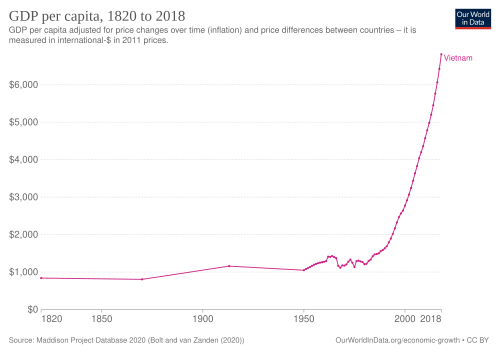
\includegraphics[width=\linewidth]{gdppercapita.png} 
        \caption*{GDP per capita development in Vietnam}
        \label{fig:gdp} 
    \end{minipage}
\end{figure}

\section{1975-1997}
The government's Second \href{https://en.wikipedia.org/wiki/Five-Year_Plans_of_Vietnam#The_Second_Five-Year_Plan_(1976%E2%80%9380)}{Five-Year Plan} (1976-1981) aimed for solid high annual growth rates in industrial and agricultural sectors and national income and sought to integrate the North and the South, but the goals were not attained. The economy remained dominated by small-scale production, low labor \href{https://en.wikipedia.org/wiki/Productivity}{productivity}, material and technological shortfalls, and insufficient food and consumer goods.\textsuperscript{[Citation needed]} The more modest\textsuperscript{[clarification needed]} goals of the \href{https://en.wikipedia.org/wiki/Five-year_plans_of_Vietnam#The_Third_Five_Year_Plan_(1981%E2%80%9385)}{Third Five-Year} Plan (1981-85) were a compromise between ideological and pragmatic factions; they emphasized the development of agriculture and industry. Efforts were also made to decentralize planning and improve the managerial skills of government officials.\textsuperscript{[Citation needed]}

After reunification in 1975, the economy of Vietnam was plagued by enormous difficulties in production, imbalances in supply and demand, inefficiencies in distribution and circulation, soaring inflation rates, and rising debt problems. Vietnam is one of the few countries in modern history to experience a sharp economic deterioration in a postwar reconstruction period.\textsuperscript{[Citation needed]} Its peacetime economy was one of the poorest in the world and had shown a negative to very slow growth in total national output as well as in agricultural and industrial production.\textsuperscript{[Citation needed]} Vietnam's gross domestic product ( GDP) in 1984 was valued at US\$18.1 billion with a per capita income estimated to be between US\$200 and US\$300 per year. Reasons for this mediocre economic performance have included\textsuperscript{[according to whom?]} severe climatic conditions that afflicted agricultural crops, bureaucratic mismanagement, elimination of private ownership, extinction of entrepreneurial classes in the South, and military occupation of Cambodia (which resulted in a cutoff of much-needed international aid for reconstruction).\textsuperscript{[Citation needed][needs update]}

From the late 1970s until the early 1990s, Vietnam was a member of the \href{https://en.wikipedia.org/wiki/Comecon}{Comecon}, and therefore was heavily dependent on trade with the \href{https://en.wikipedia.org/wiki/Soviet_Union}{Soviet Union} and its allies. Following the dissolution of the Comecon and the loss of its traditional trading partners, Vietnam was forced to liberalize trade, devalue its exchange rate to increase exports, and embark on a policy of economic development.\textsuperscript{[Citation needed][dead link]}  Between 1975 and 1994, the United States imposed a trade embargo on Vietnam, forbidding any trade during the 19-year period.

In 1986, Vietnam launched a political and economic renewal campaign (\href{https://en.wikipedia.org/wiki/%C4%90%E1%BB%95i_M%E1%BB%9Bi}{Đổi Mới}) that introduced reforms to facilitate the transition from a centralized economy to a \href{https://en.wikipedia.org/wiki/Socialist-oriented_market_economy}{socialist-oriented market economy}. \textit{Đổi Mới} combined government planning with \href{https://en.wikipedia.org/wiki/Free-market}{free-market} incentives and encouraged the establishment of private businesses and foreign investment, including \href{https://en.wikipedia.org/wiki/Foreign_direct_investment}{foreign-owned enterprises}. Furthermore, the Vietnam government stressed the necessity to lower birth rates when developing the economic and social rights of the population by implementing a policy that restricted the number of children per household to two, called the \href{https://en.wikipedia.org/wiki/Two-child_policy}{two-child policy}.\textsuperscript{[Citation needed]} By the late 1990s, the success of the business and agricultural reforms ushered in under Đổi Mới was evident. More than 30,000 private businesses had been created, the economy was growing at an annual rate of more than 7\%, and poverty was nearly halved.\textsuperscript{[Citation needed]}

Since the early 1990s, Vietnam had structurally changed away from agriculture, but without industrialisation (service-oriented globalisation).\textsuperscript{[Citation needed]}

In 1990, the state sector was the key hoped-for site of \\industrialisation.\textsuperscript{[Citation needed]} The state sector transitioned away from the processes of bottom-up commercialisation of the 1980s.\textsuperscript{[Citation needed]} This created a supply capacity. The supply capacity allowed Vietnam to avoid negative shock as Soviet aid was removed,\textsuperscript{[Citation needed]} and the supply capacity allowed the economy of Vietnam to grow rapidly in the 1990s.\textsuperscript{[Citation needed]} Its growth has averaged about 7\% annually since the 1990s, a rate second only to China.\textsuperscript{[Citation needed]}

Throughout the 1990s, exports increased by as much as 20\% to 30\% in some years. In 1999, exports accounted for 40\% of GDP, an impressive performance in the midst of the economic crisis that hit other countries in Asia. Vietnam became a member of the World Trade Organization (WTO) in 2007, which freed Vietnam from textile quotas enacted worldwide as part of the \href{https://en.wikipedia.org/wiki/Multi_Fibre_Arrangement}{Multi Fibre Arrangement} (MFA) in 1974.\textsuperscript{[Citation needed]} The MFA placed restrictions on the import by industrialized countries of textiles from developing countries. For China and other WTO members, however, textile quotas under the MFA expired at the end of 2004 as agreed in the \href{https://en.wikipedia.org/wiki/Uruguay_Round}{Uruguay Round} of trade negotiations in 1994.\textsuperscript{[Citation needed]} A 2019 study found that Vietnam's WTO entry led to substantial gains in productivity for private firms, but had no impact on state-owned enterprises. In the absence of state-owned enterprises, "the overall productivity gains would have been about 40\% larger in a counterfactual Vietnamese economy."\textsuperscript{[Citation needed]}

\section{Development since 1997}
Vietnam's economic policy following the \href{https://en.wikipedia.org/wiki/1997_Asian_Financial_Crisis}{1997 Asian Financial Crisis} has been a cautious one, emphasizing \href{https://en.wikipedia.org/wiki/Macroeconomic}{macroeconomic} stability rather than growth. While the country shifted toward a more market-oriented economy, the Vietnamese government still continues to hold a tight rein over \href{https://en.wikipedia.org/wiki/Public_sector}{major state sectors}, such as the \href{https://en.wikipedia.org/wiki/Bank}{banking} system, \href{https://en.wikipedia.org/wiki/State-owned_enterprises}{state-owned enterprises} and foreign trade.\textsuperscript{[Citation needed]} GDP growth fell to 6\% in 1998 and 5\% in 1999. The economy saw continuous real GDP growth of at least 5\% since 2000.\textsuperscript{[Citation needed]}

The signing of the \href{https://en.wikipedia.org/wiki/Bilateral_Trade_Agreement}{Bilateral Trade Agreement} (BTA) between the United States and Vietnam on July 13, 2000, was a significant milestone. The BTA provided for "normal trade relations" status of Vietnamese goods in the U.S. market. It was expected that access to the U.S. market would allow Vietnam to hasten its transformation into a \href{https://en.wikipedia.org/wiki/Manufacturing}{manufacturing}-based, \href{https://en.wikipedia.org/wiki/Export}{export}-oriented economy. Furthermore, it would attract foreign investment, not only from the U.S., but also from \href{https://en.wikipedia.org/wiki/Europe}{Europe}, Asia and other regions.\textsuperscript{[Citation needed]}

In 2001, the ruling \href{https://en.wikipedia.org/wiki/Communist_Party_of_Vietnam}{Communist Party of Vietnam} approved a 10-year economic plan that enhanced the role of the private sector, while reaffirming the primacy of the state.\textsuperscript{[Citation needed]} Growth then rose to 6\% to 7\% between 2000 and 2002 even in the midst of the global \href{https://en.wikipedia.org/wiki/Recession}{recession}, making it the world's second fastest-growing economy. At the same time, \href{https://en.wikipedia.org/wiki/Investment}{investment} grew threefold and \href{https://en.wikipedia.org/wiki/Domestic_savings}{domestic savings} quintupled.\textsuperscript{[Citation needed]}

In 2003, the private sector accounted for more than one-quarter of all industrial output.\textsuperscript{[Citation needed]} However, between 2003 and 2005, Vietnam fell dramatically in the \href{https://en.wikipedia.org/wiki/World_Economic_Forum}{World Economic Forum}'s global competitiveness report rankings, largely due to negative perceptions of the effectiveness of government institutions.\textsuperscript{[Citation needed]} Official \href{https://en.wikipedia.org/wiki/Political_corruption}{corruption} is endemic, and Vietnam lags in property rights, efficient regulation of markets, and labor and financial market reforms.\textsuperscript{[Citation needed]}

Vietnam had an average GDP growth of 7.1\% a year from 2000 to 2004. The GDP growth was 8.4\% in 2005, the second-largest in Asia, trailing only \href{https://en.wikipedia.org/wiki/China}{China}'s. The government estimated that GDP grew in 2006 by 8.17\%. According to the Minister of Planning and Investment, the government targeted a GDP growth of around 8.5\% in 2007.\textsuperscript{[Citation needed]}

On November 7, 2006, the General Council at the World Trade Organization (\href{https://en.wikipedia.org/wiki/WTO}{WTO}) approved Vietnam's accession package. On January 11, 2007, Vietnam officially became the WTO's 149th member, after 11 years of preparation, including eight years of negotiation.\textsuperscript{[Citation needed]} The country's access to the WTO was intended to provide an important boost to the economy, as it ensured that the liberalizing reforms continue and created options for trade expansion. However, the accession also brought serious challenges, requiring the economy to open up to increasing foreign competition.\textsuperscript{[Citation needed]}

Vietnam's economy continues to expand at an annual rate in excess of 7\%, one of the fastest-growing in the world, but it grew from an extremely low base, as it suffered the crippling effect of the \href{https://en.wikipedia.org/wiki/Vietnam_War}{Vietnam War} from the 1950s to the 1970s, the punitive embargoes of the United States and its allies, as well as the austerity measures introduced in its aftermath.\textsuperscript{[Citation needed]} In 2012, the communist party was forced to apologise about the mismanagement of the economy after a large number of SOEs went bankrupt and inflation rose. The main danger has been over the bad debt in the banks totalling to 15\% and forecast growth is 5.2\% for 2012 but this is also due to the global economic crisis.\textsuperscript{[Citation needed]} The government has launched schemes to reform the economy, such as lifting foreign ownership cap from 49\% and partially privatizing the country's state-owned companies that have been responsible for the recent economic downturn. By the end of 2013, the government is expected to privatize 25-50\% of SOEs, only maintaining control on public services and military. The recent reforms have created a major boom in the Vietnamese stock market as confidence in the Vietnamese economy is returning.

Vietnam's current economic turmoil has given rise to questions of a possible new period of changing political economy, however\cite{55} poverty remains to be the main concern on the national performance index as of 2018. The Provincial Governance and Public Administration Performance Index (PAPI) found that 28\% of survey respondents cited poverty as their main problem.\cite{56} Most respondents agreed with the statement that "[P]overty reduction is imperative to ensuring that Vietnam becomes an advanced, developed country. The percentage of the poorest Vietnamese respondents who believed that their economic situation would worsen increased from 13\% in 2016 to 26\% in 2017.\cite{56} The percentage of respondents with health insurance increased from 74\% in 2016 to 81\% in 2017, with strongest gains in the rural population groups.\cite{56}

In 2017, Transparency International, a non-profit that tracks \href{https://en.wikipedia.org/wiki/Graft_(politics)}{graft} ranked Vietnam as 113th worst out of 176 countries and regions for perceptions of corruption.\cite{56}\textsuperscript{\href{https://en.wikipedia.org/wiki/Wikipedia:Verifiability}{[failed verification]}} Several \href{https://en.wikipedia.org/wiki/Graft_(politics)}{graft} cases found in 2016 and 2017 led to the corruption crackdown which prosecuted many bankers, businesspeople, and government officials under charges of corruption. PAPI found that bribery at public district hospital services decreased from 17\% in 2016 to 9\% in 2017.\textsuperscript{[Citation needed]} Reports of land seizures went down from an average of about 9\% before 2013, to less than 7\% in 2017. The number of respondents who believed that their land was sold at a fair market value decreased from 26\% in 2014 to 21\% in 2017.\textsuperscript{[Citation needed]} Land-use graft and petty graft, such as police officers accepting bribes, are common. According to \href{https://en.wikipedia.org/wiki/Ralph_Jennings}{Ralph Jennings}, Vietnam has been privatizing many of its state-owned operations to reduce corruption and increase efficiency.\textsuperscript{[Citation needed][undue weight? - discuss]}

As of March 2018, Vietnam's economy continued to grow, achieving the best annual growth rate in over a decade; which has led media outlets to speculate if in the near future it could be one of the \href{https://en.wikipedia.org/wiki/Four_Asian_Tigers}{Asian tigers}.\textsuperscript{[Citation needed]}

According to \href{https://en.wikipedia.org/wiki/DBS_Bank}{DBS Bank} in 2019, Vietnam's economy has the potential to grow at a pace of about 6.0\%-6.5\% by 2029. Vietnam can overpower \href{https://en.wikipedia.org/wiki/Economy_of_Singapore}{Singapore's economy} by the next decade because of its strong foreign investment inflow and productivity growth.\textsuperscript{[Citation needed]} However, Vietnam has surpassed Singapore just a year later.

In the early 2020s, despite trade wars with Vietnam's major trade partners, a pandemic and the increasing trend in deglobalisation, Vietnam has still managed to become Asia's top-performing economy.\textsuperscript{[Citation needed]} Since 2000, Vietnam has now managed to manufacture higher-value goods with better paying jobs due to its more highly skilled workers. These workers now produce electronics which makes up 38\% (in 2020) of Vietnam's exports (compared to 14\% in 2010). The country had achieved an average of 6.2\% in economic growth (faster than any other country in Asia after China).\textsuperscript{[Citation needed]} Foreign investment on the \href{https://en.wikipedia.org/wiki/Luxury_hotel}{luxury hotels} sector and \href{https://en.wikipedia.org/wiki/Resorts}{resorts} will rise to support the \href{https://en.wikipedia.org/wiki/Tourist_industry}{tourist industry}.\textsuperscript{[Citation needed]}

\chapter{Data}
The following table shows the main economic indicators in 1990-2023 (with IMF staff estimations in 2021-2027). Inflation below 5\% is in green.

\begin{table}[htbp]
\resizebox{\textwidth}{!}{
\begin{tabular}{ccccccccc}
\rowcolor[HTML]{EAECF0} 
{\color[HTML]{202122} \textbf{Year}} & {\color[HTML]{202122} \textbf{\begin{tabular}[c]{@{}c@{}}GDP growth\\ (real)\end{tabular}}} & {\color[HTML]{202122} \textbf{\begin{tabular}[c]{@{}c@{}}GDP\\ (in Bil. US\$nominal)\end{tabular}}} & {\color[HTML]{202122} \textbf{\begin{tabular}[c]{@{}c@{}}GDP\\ (in Bil. US\$PPP)\end{tabular}}} & {\color[HTML]{202122} \textbf{\begin{tabular}[c]{@{}c@{}}GDP per capita\\ (in US\$ nominal)\end{tabular}}} & {\color[HTML]{202122} \textbf{\begin{tabular}[c]{@{}c@{}}GDP per capita\\ (in US\$ PPP)\end{tabular}}} & {\color[HTML]{202122} \textbf{\begin{tabular}[c]{@{}c@{}}Inflation rate\\ (in Percent)\end{tabular}}} & {\color[HTML]{202122} \textbf{\begin{tabular}[c]{@{}c@{}}Unemployment rate\\ (in Percent)\end{tabular}}} & {\color[HTML]{202122} \textbf{\begin{tabular}[c]{@{}c@{}}Government debt\\ (in \% of GDP)\end{tabular}}} \\
\rowcolor[HTML]{F8F9FA} 
{\color[HTML]{202122} 1990}        & {\color[HTML]{202122} 5.0}                                                                  & {\color[HTML]{202122} 8.2}                                                                          & {\color[HTML]{202122} 77.7}                                                                     & {\color[HTML]{202122} 121.7}                                                                               & {\color[HTML]{202122} 1151.2}                                                                          & {\color[HTML]{202122} 36.0}                                                                           & {\color[HTML]{202122} 12.3}                                                                              & {\color[HTML]{202122} n/a}                                                                               \\
\rowcolor[HTML]{F8F9FA} 
{\color[HTML]{202122} 1991}        & {\color[HTML]{202122} 5.8}                                                                  & {\color[HTML]{202122} 9.7}                                                                          & {\color[HTML]{202122} 85.0}                                                                     & {\color[HTML]{202122} 141.1}                                                                               & {\color[HTML]{202122} 1236.3}                                                                          & {\color[HTML]{202122} 81.8}                                                                           & {\color[HTML]{202122} 10.4}                                                                              & {\color[HTML]{202122} n/a}                                                                               \\
\rowcolor[HTML]{F8F9FA} 
{\color[HTML]{202122} 1992}        & {\color[HTML]{202122} 8.7}                                                                  & {\color[HTML]{202122} 12.5}                                                                         & {\color[HTML]{202122} 94.5}                                                                     & {\color[HTML]{202122} 179.0}                                                                               & {\color[HTML]{202122} 1350.3}                                                                          & {\color[HTML]{202122} 37.7}                                                                           & {\color[HTML]{202122} 11.0}                                                                              & {\color[HTML]{202122} n/a}                                                                               \\
\rowcolor[HTML]{F8F9FA} 
{\color[HTML]{202122} 1993}        & {\color[HTML]{202122} 8.1}                                                                  & {\color[HTML]{202122} 16.7}                                                                         & {\color[HTML]{202122} 104.6}                                                                    & {\color[HTML]{202122} 235.0}                                                                               & {\color[HTML]{202122} 1468.3}                                                                          & {\color[HTML]{202122} 8.4}                                                                            & {\color[HTML]{202122} 10.6}                                                                              & {\color[HTML]{202122} n/a}                                                                               \\
\rowcolor[HTML]{F8F9FA} 
{\color[HTML]{202122} 1994}        & {\color[HTML]{202122} 8.8}                                                                  & {\color[HTML]{202122} 20.7}                                                                         & {\color[HTML]{202122} 116.2}                                                                    & {\color[HTML]{202122} 286.0}                                                                               & {\color[HTML]{202122} 1605.0}                                                                          & {\color[HTML]{202122} 9.5}                                                                            & {\color[HTML]{202122} 10.3}                                                                              & {\color[HTML]{202122} n/a}                                                                               \\
\rowcolor[HTML]{F8F9FA} 
{\color[HTML]{202122} 1995}        & {\color[HTML]{202122} 9.5}                                                                  & {\color[HTML]{202122} 26.4}                                                                         & {\color[HTML]{202122} 130.0}                                                                    & {\color[HTML]{202122} 358.7}                                                                               & {\color[HTML]{202122} 1765.7}                                                                          & {\color[HTML]{202122} 16.9}                                                                           & {\color[HTML]{202122} 5.8}                                                                               & {\color[HTML]{202122} n/a}                                                                               \\
\rowcolor[HTML]{F8F9FA} 
{\color[HTML]{202122} 1996}        & {\color[HTML]{202122} 9.3}                                                                  & {\color[HTML]{202122} 31.4}                                                                         & {\color[HTML]{202122} 144.8}                                                                    & {\color[HTML]{202122} 419.1}                                                                               & {\color[HTML]{202122} 1934.8}                                                                          & {\color[HTML]{202122} 5.6}                                                                            & {\color[HTML]{202122} 5.9}                                                                               & {\color[HTML]{202122} n/a}                                                                               \\
\rowcolor[HTML]{F8F9FA} 
{\color[HTML]{202122} 1997}        & {\color[HTML]{202122} 8.2}                                                                  & {\color[HTML]{202122} 34.1}                                                                         & {\color[HTML]{202122} 159.3}                                                                    & {\color[HTML]{202122} 449.3}                                                                               & {\color[HTML]{202122} 2095.7}                                                                          & {\color[HTML]{202122} 3.1}                                                                            & {\color[HTML]{202122} 6.0}                                                                               & {\color[HTML]{202122} n/a}                                                                               \\
\rowcolor[HTML]{F8F9FA} 
{\color[HTML]{202122} 1998}        & {\color[HTML]{202122} 5.8}                                                                  & {\color[HTML]{202122} 34.6}                                                                         & {\color[HTML]{202122} 170.3}                                                                    & {\color[HTML]{202122} 448.1}                                                                               & {\color[HTML]{202122} 2207.3}                                                                          & {\color[HTML]{202122} 8.1}                                                                            & {\color[HTML]{202122} 6.9}                                                                               & {\color[HTML]{202122} n/a}                                                                               \\
\rowcolor[HTML]{F8F9FA} 
{\color[HTML]{202122} 1999}        & {\color[HTML]{202122} 4.8}                                                                  & {\color[HTML]{202122} 36.4}                                                                         & {\color[HTML]{202122} 181.0}                                                                    & {\color[HTML]{202122} 465.2}                                                                               & {\color[HTML]{202122} 2310.3}                                                                          & {\color[HTML]{202122} 4.1}                                                                            & {\color[HTML]{202122} 6.7}                                                                               & {\color[HTML]{202122} n/a}                                                                               \\
\rowcolor[HTML]{F8F9FA} 
{\color[HTML]{202122} 2000}        & {\color[HTML]{202122} 6.8}                                                                  & {\color[HTML]{202122} 39.6}                                                                         & {\color[HTML]{202122} 197.6}                                                                    & {\color[HTML]{202122} 498.6}                                                                               & {\color[HTML]{202122} 2489.3}                                                                          & {\color[HTML]{202122} -1.8}                                                                           & {\color[HTML]{202122} 6.4}                                                                               & {\color[HTML]{202122} 24.8}                                                                              \\
\rowcolor[HTML]{F8F9FA} 
{\color[HTML]{202122} 2001}        & {\color[HTML]{202122} 6.9}                                                                  & {\color[HTML]{202122} 41.3}                                                                         & {\color[HTML]{202122} 216.0}                                                                    & {\color[HTML]{202122} 513.2}                                                                               & {\color[HTML]{202122} 2684.5}                                                                          & {\color[HTML]{202122} -0.3}                                                                           & {\color[HTML]{202122} 6.3}                                                                               & {\color[HTML]{202122} 25.4}                                                                              \\
\rowcolor[HTML]{F8F9FA} 
{\color[HTML]{202122} 2002}        & {\color[HTML]{202122} 7.1}                                                                  & {\color[HTML]{202122} 44.6}                                                                         & {\color[HTML]{202122} 234.9}                                                                    & {\color[HTML]{202122} 546.6}                                                                               & {\color[HTML]{202122} 2881.3}                                                                          & {\color[HTML]{202122} 4.1}                                                                            & {\color[HTML]{202122} 6.0}                                                                               & {\color[HTML]{202122} 27.7}                                                                              \\
\rowcolor[HTML]{F8F9FA} 
{\color[HTML]{202122} 2003}        & {\color[HTML]{202122} 7.3}                                                                  & {\color[HTML]{202122} 50.2}                                                                         & {\color[HTML]{202122} 257.1}                                                                    & {\color[HTML]{202122} 610.4}                                                                               & {\color[HTML]{202122} 3124.4}                                                                          & {\color[HTML]{202122} 3.3}                                                                            & {\color[HTML]{202122} 5.8}                                                                               & {\color[HTML]{202122} 29.8}                                                                              \\
\rowcolor[HTML]{F8F9FA} 
{\color[HTML]{202122} 2004}        & {\color[HTML]{202122} 7.8}                                                                  & {\color[HTML]{202122} 62.9}                                                                         & {\color[HTML]{202122} 284.6}                                                                    & {\color[HTML]{202122} 757.0}                                                                               & {\color[HTML]{202122} 3426.5}                                                                          & {\color[HTML]{202122} 7.9}                                                                            & {\color[HTML]{202122} 5.6}                                                                               & {\color[HTML]{202122} 29.4}                                                                              \\
\rowcolor[HTML]{F8F9FA} 
{\color[HTML]{202122} 2005}        & {\color[HTML]{202122} 7.5}                                                                  & {\color[HTML]{202122} 73.2}                                                                         & {\color[HTML]{202122} 315.7}                                                                    & {\color[HTML]{202122} 873.1}                                                                               & {\color[HTML]{202122} 3765.8}                                                                          & {\color[HTML]{202122} 8.4}                                                                            & {\color[HTML]{202122} 5.3}                                                                               & {\color[HTML]{202122} 28.7}                                                                              \\
\rowcolor[HTML]{F8F9FA} 
{\color[HTML]{202122} 2006}        & {\color[HTML]{202122} 7.0}                                                                  & {\color[HTML]{202122} 84.3}                                                                         & {\color[HTML]{202122} 348.1}                                                                    & {\color[HTML]{202122} 996.3}                                                                               & {\color[HTML]{202122} 4114.3}                                                                          & {\color[HTML]{202122} 7.5}                                                                            & {\color[HTML]{202122} 4.8}                                                                               & {\color[HTML]{202122} 30.2}                                                                              \\
\rowcolor[HTML]{F8F9FA} 
{\color[HTML]{202122} 2007}        & {\color[HTML]{202122} 7.1}                                                                  & {\color[HTML]{202122} 98.4}                                                                         & {\color[HTML]{202122} 383.0}                                                                    & {\color[HTML]{202122} 1152.3}                                                                              & {\color[HTML]{202122} 4484.3}                                                                          & {\color[HTML]{202122} 8.3}                                                                            & {\color[HTML]{202122} 4.6}                                                                               & {\color[HTML]{202122} 32.2}                                                                              \\
\rowcolor[HTML]{F8F9FA} 
{\color[HTML]{202122} 2008}        & {\color[HTML]{202122} 5.7}                                                                  & {\color[HTML]{202122} 124.8}                                                                        & {\color[HTML]{202122} 412.5}                                                                    & {\color[HTML]{202122} 1446.6}                                                                              & {\color[HTML]{202122} 4782.9}                                                                          & {\color[HTML]{202122} 23.1}                                                                           & {\color[HTML]{202122} 2.4}                                                                               & {\color[HTML]{202122} 31.0}                                                                              \\
\rowcolor[HTML]{F8F9FA} 
{\color[HTML]{202122} 2009}        & {\color[HTML]{202122} 5.4}                                                                  & {\color[HTML]{202122} 129.0}                                                                        & {\color[HTML]{202122} 437.5}                                                                    & {\color[HTML]{202122} 1481.4}                                                                              & {\color[HTML]{202122} 5023.9}                                                                          & {\color[HTML]{202122} 6.7}                                                                            & {\color[HTML]{202122} 2.9}                                                                               & {\color[HTML]{202122} 36.3}                                                                              \\
\rowcolor[HTML]{F8F9FA} 
{\color[HTML]{202122} 2010}        & {\color[HTML]{202122} 6.4}                                                                  & {\color[HTML]{202122} 143.2}                                                                        & {\color[HTML]{202122} 471.2}                                                                    & {\color[HTML]{202122} 1628.0}                                                                              & {\color[HTML]{202122} 5357.1}                                                                          & {\color[HTML]{202122} 9.2}                                                                            & {\color[HTML]{202122} 2.9}                                                                               & {\color[HTML]{202122} 36.8}                                                                              \\
\rowcolor[HTML]{F8F9FA} 
{\color[HTML]{202122} 2011}        & {\color[HTML]{202122} 6.4}                                                                  & {\color[HTML]{202122} 171.3}                                                                        & {\color[HTML]{202122} 511.9}                                                                    & {\color[HTML]{202122} 1949.8}                                                                              & {\color[HTML]{202122} 5826.2}                                                                          & {\color[HTML]{202122} 18.7}                                                                           & {\color[HTML]{202122} 2.2}                                                                               & {\color[HTML]{202122} 35.8}                                                                              \\
\rowcolor[HTML]{F8F9FA} 
{\color[HTML]{202122} 2012}        & {\color[HTML]{202122} 5.5}                                                                  & {\color[HTML]{202122} 195.2}                                                                        & {\color[HTML]{202122} 568.4}                                                                    & {\color[HTML]{202122} 2197.6}                                                                              & {\color[HTML]{202122} 6400.2}                                                                          & {\color[HTML]{202122} 9.1}                                                                            & {\color[HTML]{202122} 2.0}                                                                               & {\color[HTML]{202122} 38.3}                                                                              \\
\rowcolor[HTML]{F8F9FA} 
{\color[HTML]{202122} 2013}        & {\color[HTML]{202122} 5.6}                                                                  & {\color[HTML]{202122} 212.7}                                                                        & {\color[HTML]{202122} 607.0}                                                                    & {\color[HTML]{202122} 2370.0}                                                                              & {\color[HTML]{202122} 6762.7}                                                                          & {\color[HTML]{202122} 6.6}                                                                            & {\color[HTML]{202122} 2.2}                                                                               & {\color[HTML]{202122} 41.4}                                                                              \\
\rowcolor[HTML]{F8F9FA} 
{\color[HTML]{202122} 2014}        & {\color[HTML]{202122} 6.4}                                                                  & {\color[HTML]{202122} 232.9}                                                                        & {\color[HTML]{202122} 660.6}                                                                    & {\color[HTML]{202122} 2566.9}                                                                              & {\color[HTML]{202122} 7281.2}                                                                          & {\color[HTML]{202122} 4.1}                                                                            & {\color[HTML]{202122} 2.1}                                                                               & {\color[HTML]{202122} 43.6}                                                                              \\
\rowcolor[HTML]{F8F9FA} 
{\color[HTML]{202122} 2015}        & {\color[HTML]{202122} 7.0}                                                                  & {\color[HTML]{202122} 236.8}                                                                        & {\color[HTML]{202122} 700.3}                                                                    & {\color[HTML]{202122} 2581.9}                                                                              & {\color[HTML]{202122} 7635.3}                                                                          & {\color[HTML]{202122} 0.6}                                                                            & {\color[HTML]{202122} 2.3}                                                                               & {\color[HTML]{202122} 46.1}                                                                              \\
\rowcolor[HTML]{F8F9FA} 
{\color[HTML]{202122} 2016}        & {\color[HTML]{202122} 6.7}                                                                  & {\color[HTML]{202122} 252.1}                                                                        & {\color[HTML]{202122} 770.9}                                                                    & {\color[HTML]{202122} 2720.2}                                                                              & {\color[HTML]{202122} 8316.2}                                                                          & {\color[HTML]{202122} 2.7}                                                                            & {\color[HTML]{202122} 2.3}                                                                               & {\color[HTML]{202122} 47.5}                                                                              \\
\rowcolor[HTML]{F8F9FA} 
{\color[HTML]{202122} 2017}        & {\color[HTML]{202122} 6.9}                                                                  & {\color[HTML]{202122} 277.1}                                                                        & {\color[HTML]{202122} 851.1}                                                                    & {\color[HTML]{202122} 2957.9}                                                                              & {\color[HTML]{202122} 9085.6}                                                                          & {\color[HTML]{202122} 3.5}                                                                            & {\color[HTML]{202122} 2.2}                                                                               & {\color[HTML]{202122} 46.3}                                                                              \\
\rowcolor[HTML]{F8F9FA} 
{\color[HTML]{202122} 2018}        & {\color[HTML]{202122} 7.2}                                                                  & {\color[HTML]{202122} 303.1}                                                                        & {\color[HTML]{202122} 934.1}                                                                    & {\color[HTML]{202122} 3201.7}                                                                              & {\color[HTML]{202122} 9867.4}                                                                          & {\color[HTML]{202122} 3.5}                                                                            & {\color[HTML]{202122} 2.2}                                                                               & {\color[HTML]{202122} 43.7}                                                                              \\
\rowcolor[HTML]{F8F9FA} 
{\color[HTML]{202122} 2019}        & {\color[HTML]{202122} 7.2}                                                                  & {\color[HTML]{202122} 331.8}                                                                        & {\color[HTML]{202122} 1021.3}                                                                   & {\color[HTML]{202122} 3439.1}                                                                              & {\color[HTML]{202122} 10584.7}                                                                         & {\color[HTML]{202122} 2.8}                                                                            & {\color[HTML]{202122} 2.2}                                                                               & {\color[HTML]{202122} 40.8}                                                                              \\
\rowcolor[HTML]{F8F9FA} 
{\color[HTML]{202122} 2020}        & {\color[HTML]{202122} 2.9}                                                                  & {\color[HTML]{202122} 346.3}                                                                        & {\color[HTML]{202122} 1064.4}                                                                   & {\color[HTML]{202122} 3548.9}                                                                              & {\color[HTML]{202122} 10907.8}                                                                         & {\color[HTML]{202122} 3.2}                                                                            & {\color[HTML]{202122} 2.5}                                                                               & {\color[HTML]{202122} 41.1}                                                                              \\
\rowcolor[HTML]{F8F9FA} 
{\color[HTML]{202122} 2021}        & {\color[HTML]{202122} 2.6}                                                                  & {\color[HTML]{202122} 370.1}                                                                        & {\color[HTML]{202122} 1141.0}                                                                   & {\color[HTML]{202122} 3756.9}                                                                              & {\color[HTML]{202122} 11589.3}                                                                         & {\color[HTML]{202122} 1.8}                                                                            & {\color[HTML]{202122} 3.2}                                                                               & {\color[HTML]{202122} 39.0}                                                                              \\
\rowcolor[HTML]{F8F9FA} 
{\color[HTML]{202122} 2022}        & {\color[HTML]{202122} 8.0}                                                                  & {\color[HTML]{202122} 408.0}                                                                        & {\color[HTML]{202122} 1321.3}                                                                   & {\color[HTML]{202122} 4101.7}                                                                              & {\color[HTML]{202122} 13284.2}                                                                         & {\color[HTML]{202122} 3.2}                                                                            & {\color[HTML]{202122} 2.3}                                                                               & {\color[HTML]{202122} 34.6}                                                                              \\
\rowcolor[HTML]{F8F9FA} 
{\color[HTML]{202122} 2023}        & {\color[HTML]{202122} 5.1}                                                                  & {\color[HTML]{202122} 433.7}                                                                        & {\color[HTML]{202122} 1438.5}                                                                   & {\color[HTML]{202122} 4324.0}                                                                              & {\color[HTML]{202122} 14324.4}                                                                         & {\color[HTML]{202122} 3.3}                                                                            & {\color[HTML]{202122} 2.0}                                                                               & {\color[HTML]{202122} 34.0}                                                                              \\
\rowcolor[HTML]{F8F9FA} 
\end{tabular}
}
\end{table}

\chapter{Economic sectors}
\section{Agriculture, fishery and forestry}

\begin{wrapfigure}{r}{.45\textwidth}
    \vspace{-25pt}
    \centering
    \begin{framed}
   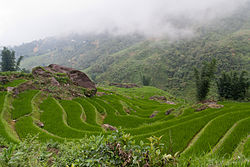
\includegraphics{250px-Sa_Pa_Rice_Terrace_IV.jpg}
    \caption*{Vietnam is the world's third-largest rice exporter.}
       \end{framed}
    \begin{framed}
    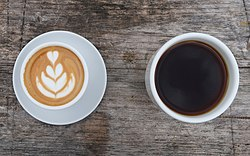
\includegraphics[width=30mm,scale=0.5]{Latte_and_dark_coffee.jpg}
    \caption*{Vietnam is the world's second-largest \href{https://en.wikipedia.org/wiki/Coffee}{coffee} producer and exporter.}
    \end{framed}
    
    \begin{framed}
    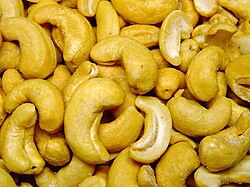
\includegraphics[width=25mm,scale=0.5]{CashewSnack.jpg}
    \caption*{Vietnam is the world's largest \href{https://en.wikipedia.org/wiki/Cashew}{cashew exporter}}    
    \end{framed}
    \vspace{-50pt}
\end{wrapfigure}

In 2003, Vietnam produced an estimated 30.7 million cubic meters of wood. Production of sawn wood was a more modest 2,950 cubic meters. In 1992, in response to \href{https://en.wikipedia.org/wiki/Deforestation_in_Vietnam}{dwindling forests}, Vietnam imposed a ban on the export of logs and raw timber. In 1997, the ban was extended to all timber products except wooden artifacts. During the 1990s, Vietnam began to reclaim land for forests with a tree-planting program.\textsuperscript{[Citation needed]}
\begin{sloppypar}\raggedright
Vietnam's \href{https://en.wikipedia.org/wiki/Fishing}{fishing industry}, which has abundant resources given the country's long coastline and extensive network of rivers and lakes, has generally experienced moderate growth. In 2003, the total catch was about 2.6 million tons. However, seafood exports increased fourfold between 1990 and 2002 to more than US\$2 billion, driven in part by \href{https://en.wikipedia.org/wiki/Shrimp}{shrimp} farms in the South and "catfish", which are a different species from their American counterparts, but are marketed in the United States under the same name. By selling vast quantities of shrimp and catfish to the U.S., Vietnam triggered antidumping complaints by the U.S., which imposed tariffs in the case of catfish and was considering doing the same for shrimp. In 2005, the seafood industry began to focus on domestic demand to compensate for declining exports.\cite{36}
\end{sloppypar}

Vietnam is one of the top rice exporting countries in the world, but the limited sophistication of small-scale Vietnamese farmers causes quality to suff\-er.\textsuperscript{[Citation needed]} Vietnam is also the world's second-largest exporter of coffee, trailing behind Brazil.\textsuperscript{[Citation needed]}

Vietnam produced in 2018:\textsuperscript{[Citation needed]}[needs update]

\begin{itemize}
    \item 44.0 million tons of \href{https://en.wikipedia.org/wiki/Rice}{rice} (\href{https://en.wikipedia.org/wiki/Rice_production_in_Vietnam}{5th largest producer in the world}, behind China, India, Indonesia and Bangladesh);
    \item 17.9 million tons of \href{https://en.wikipedia.org/wiki/Sugarcane}{sugarcane} (16th largest producer in the world);
    \item 14.8 million tons of \href{https://en.wikipedia.org/wiki/Vegetable}{vegetable};
    \item 9.8 million tons of \href{https://en.wikipedia.org/wiki/Cassava}{cassava} (7th largest producer in the world);
    \item 4.8 million tonnes of \href{https://en.wikipedia.org/wiki/Maize}{maize};
    \item 2.6 million tonnes of \href{https://en.wikipedia.org/wiki/Cashew_nut}{cashew nut} (largest producer in the world);
    \item 2.0 million tons of banana (20th largest producer in the world);
    \item 1.6 million tons of coffee (2nd largest producer in the world, only behind Brazil);
    \item 1.5 million tons of coconut (6th largest producer in the world);
    \item 1.3 million tons of sweet potato (9th largest producer in the world);
    \item 1.2 million tons of watermelon;
    \item 1.1 million tons of natural rubber (3rd largest producer in the world, behind Thailand and Indonesia);
    \item 852 thousand tons of orange (18th largest producer in the world);
    \item 779 thousand tons of mango (including mangosteen and guava);
    \item 654 thousand tons of pineapple (12th largest producer in the world);
    \item 270 thousand tons of tea (6th largest producer in the world);
\end{itemize}

In addition to smaller productions of other agricultural products.\textsuperscript{[Citation needed]}

In 2018, Vietnam was the world's 5th largest producer of \href{https://en.wikipedia.org/wiki/Pork}{pork} (3.8 million tonnes). This year the country also produced 839 thousand tons of chicken meat, 334 thousand tons of beef, 936 million liters of cow's milk, 20 thousand tons of honey, among others.\textsuperscript{[Citation needed]}

\section{Energy, mining and minerals}

\begin{wrapfigure}{r}{.5\textwidth}
    \begin{framed}
    \centering
    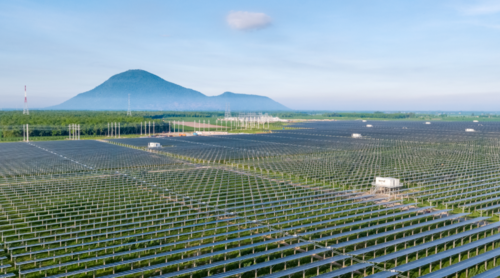
\includegraphics[width=50mm,scale=1]{Bird's_eye_view_of_installation_works_at_PV_Arrays.png}
    \caption*{\href{https://en.wikipedia.org/wiki/Dau_Tieng_Solar_Power_Project}{Dau Tieng Solar Power Complex} is the largest solar farm in \href{https://en.wikipedia.org/wiki/Southeast_Asia}{Southeast Asia}.}
    \end{framed}
\end{wrapfigure}

Petroleum is the main source of energy, followed by \href{https://en.wikipedia.org/wiki/Coal}{coal}, which contributes about 25\% of the country's energy (excluding \href{https://en.wikipedia.org/wiki/Biomass}{biomass}). Vietnam's oil reserves are in the range of 270-500 million tons. Oil production rose rapidly to 403,300 barrels per day (64,120 m3/d) in 2004, but output is believed to have peaked and is expected to decline gradually.

In 2003, mining and quarrying accounted for 9.4\% of GDP, and the sector employed 0.7\% of the workforce. Petroleum and coal are the main mineral exports. Also mined are antimony, bauxite, chromium, gold, iron, natural phosphates, tin, and zinc.\textsuperscript{[Citation needed]}

In 2019, Vietnam was the 9th largest world producer of antimony;\textsuperscript{[Citation needed]} 10th largest producer of tin;\textsuperscript{[Citation needed]} 11th largest producer of \\bauxite;\textsuperscript{[Citation needed]} 12th largest world producer of titanium;\textsuperscript{[Citation needed]} 13th largest world producer of manganese\textsuperscript{[Citation needed]} and 9th largest producer of phosphate in the world.\textsuperscript{[Citation needed]} The country is also one of the world's largest producers of ruby, sapphire, topaz and spinel.

Oil was discovered in Vietnam in the mid-1980s and oil production began in the 1990s.\textsuperscript{[Citation needed]}:24 Crude oil was Vietnam's leading export until the late 2000s, when high-tech electrical manufactures emerged to become the biggest export market (by 2014, crude oil comprised only 5\% of Vietnamese exports, compared to 20\% of all exports in 1996). This is in part because Vietnam crude oil peaked in 2004, when crude oil represented 22\% of all export earnings.\textsuperscript{[Citation needed]} Petroleum exports are in the form of crude petroleum because Vietnam has a very limited refining capacity. Vietnam's only operational refinery, a facility at Cat Hai near Ho Chi Minh City, has a capacity of only 800 barrels per day (130 m3/d). Refined petroleum accounted for 10.2\% of total imports in 2002. As of 2012, Vietnam had only one refinery, the Dung Quat refinery, but a second one, the Nghi Son Refinery was planned and was scheduled for construction in May 2013.\textsuperscript{[Citation needed]}

Vietnam's \href{https://en.wikipedia.org/wiki/Anthracite}{anthracite} coal reserves are estimated at 3.7 billion tons. Coal production was almost 19 million tons in 2003, compared with 9.6 million tons in 1999. Vietnam's potential natural gas reserves are 1.3 trillion cubic meters. In 2002, Vietnam brought ashore 2.26 billion cubic meters of natural gas. Hydroelectric power is another source of energy. In 2004, Vietnam confirmed plans to build a nuclear power plant with Russian assistance,\textsuperscript{[Citation needed]} and a second by a Japanese group.

From 2019 onwards, renewable energy deployment in Vietnam accelerated, by far surpassing the other Southeast Asian countries.\textsuperscript{[Citation needed]} Most of the newly deployed renewable energy was in the form of solar and wind power plants. By 2023, however, this development had slowed down, mainly due to limited electrical grid capacity and reduced government support.\textsuperscript{[Citation needed]}
\clearpage
\begin{table}
    Insert table of Total energy consumption in \href{https://en.wikipedia.org/wiki/Terrawatt-hour}{Terrawatt-hours} (\textbf{TWh})
    \caption*{Table 4.1}
\end{table}

\section{Industry and manufacturing}

\begin{wrapfigure}{r}{.5\textwidth}
    \begin{framed}
        Insert picture of VinFast VF8
        \caption*{\href{https://en.wikipedia.org/wiki/VinFast}{VinFast}, Vietnam's first global automaker has its manufacturing facility in \href{https://en.wikipedia.org/wiki/Haiphong}{Hải Phòng}.}
        \caption*{Figure 4.5}
    \end{framed}
\end{wrapfigure}

Although the industrial sector contributed 40.1\% of GDP in 2004, it employed only 12.9\% of the workforce. In 2000, 22.4\% of industrial production was attributable to non-state activities. From 1994 to 2004, the industrial sector grew at an average annual rate of 10.3\%. Manufacturing contributed 20.3\% of GDP in 2004, while employing 10.2\% of the workforce.

From 1994 to 2004, manufacturing GDP grew at an average annual rate of 11.2\%. The top manufacturing sectors — electronics, food processing, cigarettes and tobacco, textiles, chemicals, and footwear goods — experienced rapid growth. Benefits from its proximity to China with lower labor cost, Vietnam is becoming a new manufacturing hub in Asia, especially for Korean and Japanese firms. For instance, Samsung produces about 40\% of its phones in Vietnam.\textsuperscript{[Citation needed]}

As of 2019, Samsung employs over 200,000 employees in the Hanoi-area of Vietnam to produce \href{https://en.wikipedia.org/wiki/Smartphones}{smartphones}, while offsourcing some manufacturing to China\textsuperscript{[Citation needed]} and manufacturing large portions of its phones in Ind\-ia.\textsuperscript{[Citation needed]} \href{https://en.wikipedia.org/wiki/LG_Electronics}{LG Electronics} moved smartphone production to Vietnam from South Korea, in order to stay competitive. LG said that "Vietnam provides an "abundant labor force", as motivation for the move.\textsuperscript{[Citation needed]}

Of note, Samsung accounted for 15 percent of Vietnam's exports in the first seven months of 2024.\textsuperscript{[Citation needed]} Although significant, this is a decrease from 2017, during which Samsung accounted for 22.7 percent of Vietnam's exports.\textsuperscript{[Citation needed]}

In the past decade, a significant \href{https://en.wikipedia.org/wiki/Automotive_industry_in_Vietnam}{automotive industry} has been \\developed.\textsuperscript{[citation needed]}

\section{Services and tourism}
In 2004, services accounted for 38.2\% of gross domestic product (GDP). From 1994 to 2004, GDP attributable to the service sector grew at an average annual rate of 6.0\%
\subsection{Tourism}


\begin{wrapfigure}{r}{.65\textwidth}

    \begin{framed}
        \begin{minipage}[t]{0.5\textwidth}
            Insert photo of Ha Long Bay
            \caption*{Hạ Long Bay was recognised as a World Heritage Site in 1994.}
            \caption*{Figure 4.6}
        \end{minipage}
        \hspace{5pt}
        \begin{minipage}[t]{0.45\textwidth}
            Insert photo of Ha Nột Ancient town
            \caption*{\href{https://en.wikipedia.org/wiki/Hoi_An}{Hội An Ancient Town}}
            \caption*{Figure 4.7}
        \end{minipage}
    \end{framed}
\end{wrapfigure}

In 2012, Vietnam received 6.8 million international visitors and the number is expected to reach over 7 million in 2013. Vietnam keeps emerging as an attractive destination. In TripAdvisor's list of top 25 destinations Asia 2013 by travelers' choice, there are four cities of Vietnam, namely Hanoi, Ho Chi Minh City, Hoi An and Ha Long.\textsuperscript{[citation needed]}

2016 was the first year ever which Vietnam received over 10 million international visitors.\textsuperscript{[Citation needed]} Since then, this figure has continued to rise. In 2019, Vietnam with 18 million international visitors was fifth most visited country in the Asia-Pacific region as per World Tourism rankings released by the United Nations World Tourism Organization.\textsuperscript{[Citation needed]}

During the \href{https://en.wikipedia.org/wiki/COVID-19_pandemic_in_Vietnam}{COVID-19 pandemic in Vietnam}, the country suspended issuance of all tourist visas from March 2020 and recorded a 98\% year-on-year drop in foreign visitors for April 2020. Furthermore, Total tourism revenues dropped by over 60\% year-on-year for July 2020.\textsuperscript{[Citation needed]} The country reopened to international arrivals in March of 2022.

In the first six months of 2024, Vietnam received 6,943,961 tourist arrivals representing an increase over the same period in 2023 of 65.7 percent.\textsuperscript{[Citation needed]}

\section{Export of labour}
The export of labour, that is the sending of Vietnamese workers to work in other countries, is also key to the Vietnamese economy, with much of their earnings being sent back to Vietnam. This labour export was disrupted due to the \href{https://en.wikipedia.org/wiki/COVID-19_pandemic}{Covid pandemic}, however by 2022, Vietnam hopes to send 90,000 workers abroad. Traditional destinations have included South Korea, Japan, Malaysia, the Republic of China, and now Vietnam is aiming for Germany, Russia, and Israel.\textsuperscript{[Citation needed]}
\clearpage
\section{Banking and fiance}
\subsection{Banking}

\begin{wrapfigure}{r}{.45\textwidth}
    \begin{framed}
        Insert picture of state bank of Vietnam.
        \caption*{State Bank of Vietnam in Ho Chi Minh City (Saigon)}
        \caption*{Figure 4.8}
    \end{framed}

    \begin{framed}
        Insert picture of Ho Chi Minh's exchange tower
        \caption*{Ho Chi Minh City Stock Exchange}
        \caption*{Figure 4.9}
    \end{framed}
    \vspace{-50pt}
\end{wrapfigure}
The most important banks are the state-owned \href{https://en.wikipedia.org/wiki/Vietinbank}{VietinBank}, \href{https://en.wikipedia.org/wiki/BIDV}{BIDV}, and \href{https://en.wikipedia.org/wiki/Vietcombank}{Vietcombank}, which dominate the banking sector. There is also a trend of foreign investment into profitable banks. For example, VietinBank is currently owned by Bank of Tokyo Mitsubishi UFJ (19.73\%) while Vietcombank is owned by Mizuho (15\%).

\begin{table}[h]
    Insert table of Vietnam's top five banks\\by authorised capital
\end{table}
\textit{(NOTE: Average exchange rates of 2020. Source: tradingeconomics.com. 1 USD = 23,286 VND)}

\subsubsection{Fiance}
Vietnam has two stock trading centers, the \href{https://en.wikipedia.org/wiki/Ho_Chi_Minh_City_Securities_Trading_Center}{Ho Chi Minh City Securities Trading Center} and the \href{https://en.wikipedia.org/wiki/Hanoi_Securities_Trading_Center}{Hanoi Securities Trading Center}, which run the \href{https://en.wikipedia.org/wiki/Ho_Chi_Minh_Stock_Exchange}{Ho Chi Minh Stock Exchange} (HOSE) and the \href{https://en.wikipedia.org/wiki/Hanoi_Stock_Exchange}{Hanoi Stock Exchange} (HNX), respectively. However, there is also a third market, the Unlisted Public Companies market (UPCOM) which is a part of the Hanoi Stock Exchange. Together these two trading centres and three exchanges come under the purview of the Vietnam Stock Exchange (VSE). The VSE is a legislated body overseen by the State Securities Commission (SSC) which is a branch of the Ministry of Finance. This structure was established through the Law on Securities 2019.\textsuperscript{[Citation needed]}

\chapter{Currency, exchange rate and inflation}
\begin{wrapfigure}{r}{.45\textwidth}
    \vspace{-35pt}
    \begin{framed}

        Insert picture of Countries or territories by GDP (nominal) per capita in 2022.
        \caption*{Figure 4.10}
    \end{framed}

    \begin{framed}
        Insert picture of Countries or territories by GDP (PPP) per capita in 2022.
        \caption*{Figure 4.11}
    \end{framed}
    \vspace{-35pt}
\end{wrapfigure}


The currency used in Vietnam is the \href{https://en.wikipedia.org/wiki/%C4%90%E1%BB%93ng}{đồng}, shortened as VND or đ.    


\section{Exchange rate}

The exchange rate between the U.S. dollar and the \href{https://en.wikipedia.org/wiki/Vietnamese_%C4%91%E1%BB%93ng}{Vietnamese đồng} is important because the dong, although not freely convertible, is loosely pegged to the dollar through an arrangement known as a "\href{https://en.wikipedia.org/wiki/Crawling_peg}{crawling peg}". This mechanism allows the dollar-dong exchange rate to adjust gradually to changing market conditions.\textsuperscript{[Citation needed]} This was set at 3 percent either side of a fixed rate set each day by the SBV, however, it was increased to 5 percent in October of 2022.\textsuperscript{[Citation needed]}

As of December 27, 2024, a US dollar is worth 25,448 Vietnamese đồng.

Gold still maintains its position as a physical currency to a certain extent, although it has seen its economic role declining in recent years.\textsuperscript{[Citation needed]}
\clearpage
\section{Inflation}

Vietnam saw high inflation in 1980s.\textsuperscript{[Citation needed]} During this period, there was excessive demand for the industrial sector development, food, and other commodities. In order to stimulate supply, government attempted co-integration of parallel and planned market. Though the initial reform\textsuperscript{[Citation needed]} in the 1980s raised the total output, due to the report being partial, it also led to the CPI inflation rate being pushed to 200\% in 1982. To tackle this, the government introduced forced savings, which can be understood as the accumulation of unspent money to make the monetary overhang.[clarification needed]

Vietnam's economy experienced a \href{https://en.wikipedia.org/wiki/Hyperinflation}{hyperinflation} period in its early years of the extensive reform program, especially from 1987 to 1992.\textsuperscript{[Citation needed]}

In 2008, inflation was tracking at 20.3\% for the first half of the \\year,\textsuperscript{[Citation needed]} higher than the 3.4\% in 2000, but down significantly from 160\% in 1988.\textsuperscript{[Citation needed]}

In 2010, inflation stood at 11.5\%, and 18.58\% in 2011.\textsuperscript{[Citation needed]}

At the end of 2012, inflation stood at 7.5\%, a substantial decrease from 20\-11.\textsuperscript{[Citation needed]}

In 2013, inflation stood at 6\%,\textsuperscript{[Citation needed]} and 4.09\% in 2014.\textsuperscript{[Citation needed]} In 2016, it was only 2\%.

\chapter{Merges and acquisitions}

With 1,120 inbound deals with a cumulated value of almost 15 billion USD, there is a demonstrated interest by foreign companies to access the Vietnamese market or continue expansion using \href{https://en.wikipedia.org/wiki/Mergers_and_acquisitions}{mergers and acquisitions}. From 1991 to February 2018, Vietnamese companies were involved as either an acquiror or an acquired company in 4,000 mergers and acquisitions with a total value of 40.6 billion USD. The mergers and acquisitions activities faced many obstacles, lowering the rate of success of the transaction. Common obstacles come from culture, transparency and legal aspects.\textsuperscript{[Citation needed]} The Institute for Mergers, Acquisitions and Alliances that has been active in Vietnam since 2006 and its M\&A expert Christopher Kummer think that after the peak in 2016 and 2017 the trend will decrease in 2018.\textsuperscript{[Citation needed]} Among the largest and most prominent transactions since 2000 are:

\begin{table}[h]
    \centering
    Insert table of some of the largest and most prominent transactions since 2000
\end{table}

\chapter{Trade}

\begin{wrapfigure}{r}{.35\textwidth}
    \begin{framed}
        Insert picture of Saigon Port
        \caption*{\href{https://en.wikipedia.org/wiki/Saigon_Port}{Saigon Port} is the \href{https://en.wikipedia.org/wiki/List_of_busiest_container_ports}{busiest container port} in Vietnam. It is capable of accommodating \href{https://en.wikipedia.org/wiki/Panamax}{post-Panamax} ships.}
        \caption*{Figure 7.1}
    \end{framed}
\end{wrapfigure}

Economic relations with the United States are improving but are not without challenges. Although the United States and Vietnam reached a landmark bilateral agreement in December 2001, which helped increase Vietnam's exports to the United States, disagreements over textile and catfish exports are hindering full implementation of the agreement. Further disrupting the economic relations between the two countries were efforts in Congress to link non-humanitarian aid to Vietnam's human rights record. Barriers to trade and intellectual property are also within the purview of bilateral discussions.\textsuperscript{[Citation needed]}

Given neighboring China's rapid economic ascendancy, Vietnam highly values its economic relationship with China. Following the resolution of most territorial disputes, trade with China is growing rapidly, and in 2004, Vietnam imported more products from China than from any other country. In November 2004, the \href{https://en.wikipedia.org/wiki/Association_of_Southeast_Asian_Nations}{Association of Southeast Asian Nations} (ASEAN), of which Vietnam is a member, and China announced plans to establish the world's largest free-trade area by 2010.\textsuperscript{[Citation needed]}

Vietnam became a member of the \href{https://en.wikipedia.org/wiki/World_Trade_Organization}{World Trade Organization} (WTO) on January 11, 2007.\textsuperscript{[Citation needed]}

In December 2015, Vietnam joined the \href{https://en.wikipedia.org/wiki/ASEAN_Economic_Community}{ASEAN Economic Community} along with the 9 other ASEAN members. The community's goal is to integrate the 10 members of ASEAN and bring a freer flow of labor, investment and trade to the region.\textsuperscript{[Citation needed]}

Currently, Vietnam is being tugged in multiple directions from multiple powers, namely, Russia, China and the U.S. in its attempts to achieve economic multilateralization.\textsuperscript{[Citation needed]} Alternatively in the region, it is also pulled by either China, South Korea, Japan or ASEAN countries, as well as other constituents such as Taiwan \& Hong Kong as well as Australia/New Zealand and India in the region (\href{https://en.wikipedia.org/wiki/ASEAN#Relations_with_other_blocs}{ASEAN+3 and ASEAN+6}).\textsuperscript{[Citation needed]}

\section{Foreign Trade}
Since \href{https://en.wikipedia.org/wiki/%C4%90%E1%BB%95i_M%E1%BB%9Bi}{Đổi Mới} in 1986, Vietnam has increased trading, growing both exports and imports in double digits ever since. More recently, alarms on trade account deficits have been raised domestically, especially after joining the WTO in 2007. Throughout the next five years after 2007, Vietnam ran a trade deficit with the rest of the world in the tens of billions of dollars, with the record trade deficit in 2008 of US\$18 billion.\textsuperscript{[Citation needed]}

The account deficit has since decreased. In 2012, Vietnam recorded a trade surplus of US\$780 million, the first trade surplus since 1993. Total trade reached US\$228.13 billion, an increase of 12.1\% from 2011.\textsuperscript{[Citation needed]} In 2013, Vietnam recorded the second year of trade surplus of US\$863 million. In 2014, Vietnam recorded the third year of trade surplus of US\$2.14 billion, the largest trade surplus ever in history.\textsuperscript{[Citation needed]} Three years later, in 2017, it surpassed itself with a record of \$2.92 billion.

\begin{table}[h]
    \centering
    Insert table of foreign trade of Vietnam
    \caption*{Table 7.1}
\end{table}

\subsection{Exports}

\begin{wrapfigure}{r}{.35\textwidth}
    \begin{framed}
        Insert the map of Vietnamese export destinations, 2004
        \caption*{Figure 7.2}
    \end{framed}

\end{wrapfigure}

In 2004, Vietnam's exports of merchandise were valued at US\$26.5 billion, and were growing rapidly along with imports. Vietnam's principal exports were crude oil (22.1\%), textiles and garments (17.1\%), footwear (10.5\%), fisheries products (9.4\%) and electronics (4.1\%). The main destinations of Vietnam's exports were the United States (18.8\%), Japan (13.2\%), China (10.3\%), Australia (6.9\%), Singapore (5.2\%), Germany (4.0\%), and the United Kingdom (3.8\%).\textsuperscript{[Citation needed]}

In 2012, export rose 18.2\%, valued at US\$114.57 billion.\textsuperscript{[Citation needed]} Vietnam's main export market included the EU with US\$20 billion, United States with US\$19 billion, ASEAN with \$US 17.8 billion, Japan with US\$13.9 billion, China with US\$14.2 billion, and South Korea with US\$7 billion.\textsuperscript{[Citation needed]}

In 2013, exports rose 15.4\%, valued at US\$132.17 billion, of which export of electronics now comprised 24.5\% of total export, compared with a 4.4\% in 2008. Textiles and garments are still an important part in Vietnam's export, valued about US\$17.9 billion in 2013.

In 2014, exports rose 13.6\%, reaching US\$150.1 billion. Electronics and electronics parts, textiles and garments, computers and computer parts are the three main export groups of Vietnam. The United States continued to be Vietnam's largest export market, with US\$28.5 billion. The EU is second with US\$27.9 billion, ASEAN is third, China is fourth and Japan is the fifth largest export market of Vietnam.

In 2024, Vietnam's exports increased 14.3 percent. Among Vietnam's biggest exports were garments and textiles (US\$37 billion), electronics (US\$72.6 billion), plastics (US\$11.8 billion) and furniture (US\$3.4 billion).\textsuperscript{[Citation needed]}

\subsection{Imports}

In 2004, Vietnam's merchandise \href{https://en.wikipedia.org/wiki/Import}{imports} were valued at US\$31.5 billion and growing rapidly. Vietnam's principal imports were machinery (17.5\%), refined petroleum (11.5\%), steel (8.3\%), material for the textile industry (7.2\%), and cloth (6.0\%). The main origins of Vietnam's imports were China (13.9\%), Taiwan (11.6\%), Singapore (11.3\%), Japan (11.1\%), South Korea (10.4\%), Thailand (5.8\%), and Malaysia (3.8\%).\textsuperscript{[Citation needed]}

Vietnam import rose 6.6\% in 2012, valued at US\$113.79 billion.\textsuperscript{[Citation needed]} Major import countries were China US\$29.2 billion, ASEAN with US\$22.3 billion, South Korea with US\$16.2 billion, Japan with US\$13.7 billion, EU with US\$10 billion, and United States with US\$6.3 billion.\textsuperscript{[Citation needed]}

In 2014, imports rose 12.1\%, reaching US\$148 billion, most of which are materials and machinery needed for export. China continued to be Vietnam's largest import partner, with US\$43.7 billion. The ASEAN is second with US\$23.1 billion, South Korea is third, Japan is fourth and the EU is the fifth largest import partner of Vietnam.

\section{External debt, foreign aid and foreign investment}

In 2004, external debt amounted to US\$16.6 billion, or 37\% of GDP.\textsuperscript{[Citation needed]}

From 1988 to December 2004, cumulative foreign direct investment (FDI) commitments totaled US\$46 billion. By December 2004, about 58\% had been dispersed. About half of FDI has been directed at the two major cities (and environs) of Ho Chi Minh City and Hanoi. In 2003, new foreign direct investment commitments were US\$1.5 billion. The largest sector by far for licensed FDI is industry and construction. Other sectors attracting FDI are oil and gas, fisheries, construction, agriculture and forestry, transportation and communications, and hotels and tourism. From 2006 to 2010, Vietnam hoped to receive US\$18 billion of FDI to support a targeted growth rate in excess of 7\%. Despite rising investments, foreign investors still regard Vietnam as a risky destination, as confirmed by recent survey by the Japan External Trade Organization of Japanese companies operating in Vietnam. Many of the respondents complained about high costs of utilities, office rentals and skilled labor. Corruption, bureaucracy, lack of transparent regulations and the failure to enforce investor rights are additional obstacles to investment, according to the U.S. State Department. Vietnam tied with several nations for the 102nd place in Transparencies International's Corruption Perceptions Index in 2004.\textsuperscript{[Citation needed]} A study was conducted to examine the effect foreign investment had on corruption in Vietnam. The study concluded that the propensity of foreign firms to bribe at entry is higher in restricted sectors. Also, the removal of investment restrictions leads to reductions in bribery as a result of more Foreign Investment Enterprises, and consequently more competition entering that sector.\textsuperscript{[Citation needed]}

The \href{World Bank}'s assistance program for Vietnam has three objectives: to support Vietnam's transition to a market economy, to enhance equitable and sustainable development and to promote good governance. From 1993 through 2004, Vietnam received pledges of US\$29 billion of official development assistance (ODA), of which about US\$14 billion, or 49\%, has been disbursed. In 2004, international donors pledged ODA of US\$2.25 billion, of which US\$1.65 billion actually was disbursed. Three donors accounted for 80\% of disbursements in 2004: Japan, the World Bank, and the Asian Development Bank. From 2006 to 2010, Vietnam hopes to receive US\$14 billion to US\$15 billion of ODA.\textsuperscript{[Citation needed]}

Pledged foreign direct investment was US\$21.3 billion for 2007 and a record US\$31.6 billion for the first half of 2008.\textsuperscript{[Citation needed]} Mergers and acquisitions have gradually become an important channel of investments in the economy, especially after 2005.

In 2023, Vietnam realised foreign direct investment in the amount of US\$23.2 billion and recorded a further US\$36.6 billion in registered FDI commitme\-nts.\textsuperscript{[Citation needed]}

\clearpage
\section{Free trade agreements}

\begin{figure}[ht!]
    \begin{minipage}{0.49\textwidth}
        \centering
        \begin{itemize}
            \item \href{https://en.wikipedia.org/wiki/ASEAN_Free_Trade_Area}{ASEAN Free Trade Area} (AF\-TA)
            \item \href{https://en.wikipedia.org/wiki/ASEAN%E2%80%93Australia%E2%80%93New_Zealand_Free_Trade_Area}{ASEAN-Aus\-tra\-li\-a-New Zea\-land Free Trade A\-rea} (A\-A\-N\-Z\-F\-T\-A) is a free trade a\-rea be\-tween A\-SEAN and A\-N\-Z\-C\-E\-R\-T\-A, sign\-ed on 27 Feb\-ruary 20\-09\textsuperscript{[Citation needed]} and com\-ing into ef\-fect on 1 Jan\-uary 20\-10.\textsuperscript{[Citation needed]} De\-tails of the A\-A\-N\-Z\-F\-T\-A agree\-ment are a\-vail\-able on\-line.\textsuperscript{[Citation needed]}
        \end{itemize}
    \end{minipage}
    \hfill
    \begin{minipage}{0.45\textwidth}
        \begin{framed}
            Insert photo of A map of A\-SEAN-China Free Trade Area including Vietnam, other free trade deals are with the European Union, Japan, Korea, the Eurasian Economic U\-nion (Russia), India, Australia, New Zealand, Canada, México, Peru and Chile
            \caption*{Figure 7.3}
        \end{framed}
    \end{minipage}
\end{figure}

\begin{itemize}
    \vspace{-5pt}
    \item ASEAN-China Free Trade Area (ACFTA), in effect as of 1 January 2010\textsuperscript{[Citation needed]}
    \item ASEAN-India Free Trade Area (AIFTA), in effect as of 1 January 20\-10\textsuperscript{[Citation needed]}
    \item ASEAN-Japan Comprehensive Economic Partnership (AJCEP)
    \item ASEAN-Korea Free Trade Area (AKFTA), in effect as of 1 January 2010\textsuperscript{[Citation needed]}
    \item Comprehensive Economic Partnership for East Asia
    \item Comprehensive and Progressive Agreement for Trans-Pacific Partnership.
    \item On 29 May 2015, Vietnam signed a Free Trade Agreement (FTA) with Eurasian Economic Union.\textsuperscript{[Citation needed]}
    \item European Union-Vietnam Free Trade Agreement (EVFTA) came into effect on 1 August 2020.
    \item Vietnam-Chile Free Trade Agreement (VCFTA) came into effect on 1 January 2014.\textsuperscript{[Citation needed]}
    \item Vietnam-Korea Free Trade Agreement (VKFTA) came into effect on 20 December 2015.\textsuperscript{[Citation needed]}
    \item Japan-Vietnam Economic Partnership Agreement came into effect on 1 October 2009.\textsuperscript{[Citation needed]}
    \item United Kingdom-Vietnam Free Trade Agreement came into effect on 1 January 2021.\textsuperscript{[Citation needed]}
\end{itemize}



\chapter{Economic development strategy}
\section{Trade liberalization}
\small{
    Over the past 30 years, Vietnam has signed numerous trade agreements with different partners, promoting the country as one of the main manufacturing hubs in the world. In 1995, Vietnam joined the ASEAN community. In 2000, it signed a free trade agreement with the United States, to be followed by admission to the World Trade Organisation in 2007. Since then, the country has further integrated itself into the world economy with bilateral agreements with other ASEAN countries, China, India, Japan, and Korea, to name a few. Vietnam has actively working with other partners on ratifying the Trans-Pacific Partnership to form CP TPP, or TPP-11, after the withdrawal of the US, in order to promote economic cooperation, regional connectivity and promote economic growth between member countries. The World Bank estimates that the CP TPP would help the country's GDP to grow by 1.1\% by 2030 with a boost to productivity. The overall impact of these efforts was the lowering of tariffs on both imports and exports to and from Viet Nam, and an improved trade balance with a surplus of \$2.8 billion during the first eight months of 2018 (Vietnam Custom Department).\textsuperscript{[Citation needed]} Most recently, on June 30, 2019, Vietnam signed the Free Trade Agreement and Investment Protection Agreement with the EU after 10 years of negotiation, making it only the fourth country in Asia which managed to sign such agreement with the western bloc (after Japan, South Korea, and Singapore)
}
\section{Domestic Reform}
The government has made real effort in changing its mindset toward a more open market economy, lowering the cost of doing business, and putting regulation in place to ensure rights and orders. In 1986 the government passed its first Law on Foreign Investment, allowing foreign companies to operate in Vietnam. Between 1981 and 2005, Vietnam created a new intellectual property law that gradually moved away from the Soviet-style concept of collective ownership.\textsuperscript{[Citation needed]} A milestone in this evolution was the Copyright Agreement that Vietnam concluded with the US in 1997, serving primarily the US interest of preventing Vietnam from becoming an international center for illegal copying.\textsuperscript{[Citation needed]} The constitution has come a long way since, with the law being revised regularly to cater for a more investor-friendly business environment while aiming to reduce red-tape and accelerate foreign investment into the country. The Global Competitiveness Report\textsuperscript{[Citation needed]} by World Economic Forum placed Vietnam at 55th in 2017, rising from 77th place in 2006. In the World Bank's Ease of Doing Business rankings,\textsuperscript{[Citation needed]} Vietnam also rose from 104th place in 2007 to 68th place in 2017. The Bank commended Vietnam on progress made in enforcing contracts, increasing access to credit and basic infrastructure, and trading, among other factors.
\section{Human and physical capital investment}
Vietnam invested a lot in its human capital and infrastructure. With a growing population - 100 million as of 2024, up from 60 million in 1986, and more than half are under the age of 35- Vietnam made large public investments in education, especially making primary education universal and compulsory. This was necessary, given the country's export-led growth strategy, where literacy for the mass workforce is deemed important for growth in the manufacturing sector. On the other hand, Vietnam also invested heavily in infrastructure, ensuring cheap mass access to necessities like electricity, water, and especially the internet. These two factors together helped Vietnam to become a hub for foreign investment and manufacturing in Southeast Asia. Japanese and Korean electronics companies like Samsung, LG, Olympus, and Pioneer built factories, and countless European and American apparel makers set up textile operations in the country. Intel opened a \$1 billion chip factory in 2010, signalling the importance of Vietnam's strategic positioning in the eyes of the international business community.

\section{Sustainable growth}
Economic growth in Vietnam was considered as broadly in line with other developing countries. The Inclusive Development Index\textsuperscript{[Citation needed]} by WEF put Vietnam in a group of countries that have done particularly well and advancing in the ranking of the world's most inclusive economies. This has been notably evident with the role of women participating in the economy. Their labor force participation rate is within 10\% of that of men, a smaller gap than many other countries according to World Bank, and in 2015 women-led households are generally not poorer than those led by men. Primary and secondary enrollment rates for boys and girls are also essentially the same, and more girls continue studying in high school than boys. The government is actively reviewing and adjusting its policy, as shown in the current official Development Strategy Action Plan 2011-2020, to develop appropriate mechanisms for a more equitable growth across the country; promoting the advantages of each regions, working in collaboration with each other to support and amplify the fruit of development.

In 2017, with the help of the United Nations, Vietnam official started the ground work to achieve the Sustainable Development Goals with the development of the "One Strategic Plan",\textsuperscript{[Citation needed]} integrating the SDGs with the nation's Socio-Economic Development Strategy (2011-2020) and Socio-Economic Development Plan (2016-2020). The OSP can be used as a guideline for government agencies to implement the SDGs in the most effective ways, focusing on areas of importance, such as: investing in people, climate resilience and environmental sustainability, prosperity and partnership, justice and inclusive governance. Vietnam has also developed a National Action Plan to review current growth policies and update these to align with the interest of the SDGs. This is done in consultation with ministries, local governments, and other stakeholders so that a common framework can be set forward.

\chapter{Economic indicators and international rankings}

\begin{center}
    \begin{tabular}{|>{\raggedright\arraybackslash}m{2.75cm} | >{\raggedright\arraybackslash}m{3.3cm} | c | >{\raggedright\arraybackslash}m{2.05cm}|}
        \hline
        \rowcolor{gray!30}
        Organization                                        & Title                                 & Year & Ranking                             \\ [0.5ex]
        \hline
        BSA (The Software Alliance)                         & The IT Industry Competitiveness Index & 2011 & 53 out of 66                        \\
        \hline
        International Monetary Fund                         & Gross Domestic Product (PPP)          & 2020 & 23 out of 190                       \\
        \hline
        World Economic Forum                                & Global Competitiveness                & 2019 & 67 out of 141                       \\
        \hline
        World Bank                                          & Ease of Doing Business                & 2018 & 68 out of 190                       \\
        \hline
        The Heritage Foun\-dation/The Wall St\-reet Journal & Index of Economic Freedom             & 2019 & 128 out of 180-mostly unfree (2019) \\
        \hline
        Transparency International                          & Corruption Perceptions Index          & 2019 & 96 out of 177                       \\
        \hline
    \end{tabular}
\end{center}
\centering Table 8.1

\chapter{Notes}

1. official data; data cover general government debt and include debt instruments issued (or owned) by government entities other than the treasury; the data include treasury debt held by foreign entities; the data include debt issued by subnational entities, as well as intragovernmental debt; intragovernmental debt consists of treasury borrowings from surpluses in the social funds, such as for retirement, medical care, and unemployment; debt instruments for the social funds are not sold at public auctions

\backmatter
\begingroup\sloppy
\begin{multicols}{2}
\begin{thebibliography}{999}\RaggedRight

\bibitem{1}"WEO Groups and Aggregates Information April 2020",\emph{World Economic and Financial Surveys World Economic Outlook Database},International Monetary Fund,6 May 2020.
\bibitem{2} "World Bank Country and Lending Groups", World Bank, 10 October 2023.
\bibitem{3} Cling, Jean-Pierre; Razafindrakoto, Mireille; Roubaud, François (Spring 2013), ``Is the World Bank compatible with the socialist-oriented market economy?'', \textit{Revue de la régulation: Capitalisme, institutions, pouvoirs}, \textbf{13} (13). \url{https://doi.org/10.4000/regulation.10081}.\par
\bibitem{4}  General Statistics Office of Vietnam (2023). \textit{Niên giám Thống kê Việt Nam năm 2022 [Statistical Yearbook of Vietnam 2022]} (PDF). Statistical Publishing House (Vietnam). p. 103. Archived (PDF) from the original on 2023-07-10. Retrieved 2023-07-10.
\bibitem{5} International Monetary Fund. \url{https://www.imf.org/external/datamapper/profile/VNM}.
\bibitem{6} "The outlook is uncertain again amid financial sector turmoil, high inflation, ongoing effects of Russia's invasion of Ukraine, and three years of COVID". International Monetary Fund. April 11, 2023.
\bibitem{7} "Vietnam's gross domestic product (GDP) growth is forecast to moderate to 5.8\% in 2025 due to increased trade policy uncertainty, according to the World Bank (WB)'s latest East Asia and Pacific Economic Update". VneExpress International. April 15, 2025.
\bibitem{8} "In the long-term, the Vietnam GDP Annual Growth Rate is projected to trend around four percent in 2026". International Monetary Fund. April 2025.
\bibitem{9} "Vietnam". CIA World Factbook.
\bibitem{10} "World Economic Outlook Database, October 2022". IMF.org. International Monetary Fund. Retrieved 2023-01-04.
\bibitem{11} "Poverty headcount ratio at \$8.30 a day (2021 PPP) (\% of population) - Vietnam". World Bank. Retrieved 13 August 2025.
\bibitem{12} "GINI index (World Bank estimate)". World Bank. Retrieved 21 March 2020.
\bibitem{13} "Human Development Report 2025". United Nations Development Programme. 6 June 2025.
\bibitem{14} "Labor force, total - Vietnam". World Bank. Retrieved 11 January 2020.
\bibitem{15} "Employment to population ratio, 15+, total (\%) (national estimate) - Vietnam". World Bank. Retrieved 11 January 2020.
\bibitem{16} General Statistics Office of Vietnam (2023). Niên giám Thống kê Việt Nam năm 2022 [Statistical Yearbook of Vietnam 2022] (PDF). Statistical Publishing House (Vietnam). pp. 99-100. Archived (PDF) from the original on 2023-07-10. Retrieved 2023-07-10.
\bibitem{17} "Unemployment, youth total (\% of total labor force ages 15-24) (national estimate) - Vietnam". World Bank \& ILO. Retrieved 7 July 2020.
\bibitem{18} "Report on Labor Force Survey Quarter 1 2024". Vietnam General Statistics Office. First Quarter 2024.
\bibitem{19} General Department of Vietnam Customs (2024). Statistics of Exports by Country/Territory (PDF). General Department of Vietnam Customs. Retrieved 25 February 2025.
\bibitem{20} General Department of Vietnam Customs (2024). Statistics of Imports by Country/Territory (PDF). General Department of Vietnam Customs. Retrieved 25 February 2025.
\bibitem{21} "The World Factbook". CIA.gov. Central Intelligence Agency. Retrieved 15 March 2019.
\bibitem{22} "Viet Nam's public debt falls to 37\% in 2023". National Institute for Finance. 1 January 2024.
\bibitem{23} "Vietnam Foreign Exchange Reserves". CEIC. Retrieved 28 February 2020.
\bibitem{24} "Sovereigns rating list". Standard \& Poor's. Archived from the original on 3 January 2013. Retrieved 18 February 2013.
\bibitem{25} Rogers, Simon; Sedghi, Ami (15 April 2011). "How Fitch, Moody's and S\&P rate each country's credit rating". Reuters. Archived from the original on 1 May 2013. Retrieved 28 September 2012.
\bibitem{26} Shriek, David K. (27 January 1974). "South Vietnam, a U. S. Subsidiary". The New York Times. ISSN 0362-4331. Retrieved 29 September 2023.
\bibitem{27} Prybyla, Jan S. (1966). "Soviet and Chinese Economic Aid to North Vietnam". The China Quarterly. 27. Cambridge University Press: 84-100. doi:10.1017/S0305741000021706.
\bibitem{28} "The World in 2050" (PDF). PricewaterhouseCoopers. February 2017. Retrieved 24 April 2017.
\bibitem{29} Ngô Sĩ Liên 1993, Đại Việt sử ký toàn thư, vol 4.
\bibitem{30} "10th-century Egyptian and Muslim ceramics found in Hanoi". Hoàng thành Thăng Long. 8 August 2013.
\bibitem{31} Hoàng Anh Tuấn (2007). Silk for Silver: Dutch-Vietnamese Relations, 1637-1700. Brill. ISBN 978-90-04-15601-2.
\bibitem{32} "Urbanization: expanding opportunities, but deeper divides". United Nations Department of Economic and Social Affairs. Retrieved 2023-06-28.
\bibitem{33} "Rise of Industrial America, 1876-1900: City Life in the Late 19th Century". U.S. History Primary Source Timeline. Classroom Materials at the Library of Congress. Library of Congress. Retrieved 2023-06-28.
\bibitem{34} Lockard, Craig A. (Fall 1994). "Meeting Yesterday Head-on: The Vietnam War in Vietnamese, American, and World History". Journal of World History. 5 (2): 227-270. ISSN 1045-6007. JSTOR 20078600.
\bibitem{35} Nguyen, Thi Ha Thanh (2009). "European Trade on the Far East and the Mercantile Relationship with Vietnam from the 16th to 19th Century". Higashi Ajia bunka kōshō kenkyū \begin{CJK*}{UTF8}{min}東アジア文化交渉研究\end{CJK*} [Cultural Approaches to East Asian Studies]. 2009 (2): 353-366.
\bibitem{36} Ronald J. Cima, ed. (1989). Vietnam: A Country Study. Library of Congress Country Studies. hdl:loc.gdc/cntrystd.vn. LCCN 88600482.
\bibitem{37} Cosslett, Tuyet L.; Shaw, William R. (1989). "The Economy - Historical Background". In Ronald J. Cima (ed.). Vietnam: A Country Study. Library of Congress Country Studies. Retrieved 3 March 2015.
\bibitem{38} "Overview: Vietnam". World Bank. April 14, 2023. Archived from the original on June 28, 2023. Retrieved June 28, 2023.
\bibitem{39} Krueger, Anne O. "The World Economy at the Start of the 21st Century". International Monetary Fund. Retrieved 2023-06-28.
\bibitem{40} Ronald J. Cima, ed. (1987). "The Economy". Vietnam: A Country Study. Library of Congress Country Studies. Washington DC: Library of Congress. Retrieved 3 March 2015.
\bibitem{41} Council Of Ministers (March 1989). "Vietnam's New Fertility Policy". Population and Development Review. 15 (1): 169-172. doi:10.2307/1973424. JSTOR 1973424.
\bibitem{42} Fforde, A. (2016). "Vietnam: Economic Strategy and Economic Reality". Journal of Current Southeast Asian Affairs. 35 (2): 3-30. doi:10.1177/186810341603500201.
\bibitem{43} Mesa-Lago, Carmelo (2025). Comparing Socialist Approaches: Economics and Social Security in Cuba, China, and Vietnam. Pitt Latin American Series. Pittsburgh, PA: University of Pittsburgh Press. ISBN 9780822948476.
\bibitem{44} "Accessions: Viet Nam". World Trade Organization. Retrieved 2022-11-20.
\bibitem{45} Baccini, Leonardo; Impullitti, Giammario; Malesky, Edmund J. (2019). "Globalization and state capitalism: Assessing Vietnam's accession to the WTO" (PDF). Journal of International Economics. 119: 75-92. doi:10.1016/j.jinteco.2019.02.004. S2CID 158525166.
\bibitem{46} Vuong, Quan-Hoang (February 2010). Financial Markets in Vietnam's Transition Economy: Facts, Insights, Implications. Saarbrücken: VDM Verlag. ISBN 978-3-639-23383-4.
\bibitem{47} "Recovery from the Asian Crisis and the Role of the IMF". International Monetary Fund. IMF Issues Briefs. May 2000. Retrieved 2023-07-14.
\bibitem{48} "Economic Growth of Viet Nam". Nerd Economics. 18 July 2020. Retrieved 2023-06-28.
\bibitem{49} "Approval of the extension of nondiscriminatory treatment with respect to the products of the Socialist Republic of Vietnam". United States House of Representatives. 5 September 2001. House Report 107-198. Retrieved 2023-06-28.
\bibitem{50} Virmani, Arvind (July 2012). "Accelerating And Sustaining Growth: Economic and Political Lessons" (PDF). IMF Working Paper 12/185. Archived (PDF) from the original on June 28, 2023.
\bibitem{51} Vuong, Quan Hoang; Tran, Tri Dung (15 June 2009). "Financial Turbulences in Vietnam's Emerging Economy: Transformation over 1991-2008 Period". Contemporary Issues in Finance. SSRN 1486204.
\bibitem{52} "Accessions: Viet Nam". World Trade Organization.
\bibitem{53} "Global Trade Liberalization and the Developing Countries". International Monetary Fund. IMF Issues Briefs. November 2001. Retrieved 2023-06-28.
\bibitem{54} "Vietnam will struggle to meet 2012 growth target". Business Week. Bloomberg. 22 October 2012. Archived from the original on 2012-10-26. Retrieved November 4, 2012.
\bibitem{55} Vuong, Quan-Hoang (16 May 2014). "Vietnam's political economy: a discussion on the 1986-2016 period". Working Papers CEB.
\bibitem{56} "Report paints brighter picture of corruption control in Vietnam". VnExpress International. Retrieved 2018-04-08.
\bibitem{57} Jennings, Ralph (19 December 2017). "Vietnam's Corruption Crackdown Is All About Protecting Its Economic Miracle From Its SOEs". Forbes.
\bibitem{58} "Vietnam's economy expands 7.38\%, best rate in a decade". The Business Times. 30 March 2018. Archived from the original on 23 September 2018. Retrieved 23 September 2018.
\bibitem{59} "Vietnam, Asia's newest 'tiger' economy, roars in 2018: QNB". Gulf Times. 11 August 2018. Archived from the original on 23 September 2018. Retrieved 23 September 2018.
\bibitem{60} "Vietnam's Economy Could Soon Be Bigger Than Singapore's". Bloomberg. 28 May 2019. Retrieved 28 May 2019.
\bibitem{61} Lee, Yen Nee (2021-01-28). "This is Asia's top-performing economy in the Covid pandemic — it's not China". CNBC. Retrieved 2022-01-21.
\bibitem{62} "Vietnam is emerging as a winner from the era of deglobalisation". The Economist. ISSN 0013-0613. Retrieved 2022-10-04.
\bibitem{63} "Room remains for growth in luxury hotel segment". Vietnam Investment Review. August 26, 2016. Archived from the original on December 20, 2019. Retrieved December 20, 2019.
\bibitem{64} "World Economic Outlook Database, April 2024". International Monetary Fund. Retrieved 2024-09-15.
\bibitem{65} Rosen, Elisabeth (24 April 2014). "Why Can't Vietnam Grow Better Rice?". The Diplomat. Retrieved 26 April 2014.
\bibitem{66} "Coffee Exports by Country". World's Top Exports. Retrieved 3 March 2015.
\bibitem{67} "Crops and livestock products". FAOSTAT. Food and Agriculture Organization of the United Nations. Retrieved 2022-11-20.
\bibitem{68} Nguyen, Phuong Anh; Abbott, Malcolm; Nguyen, Thanh Loan T. (1 April 2019). "The development and cost of renewable energy resources in Vietnam". Utilities Policy. 57: 59-66. Bibcode:2019UtPol..57...59N. doi:10.1016/j.jup.2019.01.009. ISSN 0957-1787. Retrieved 5 February 2025.
\bibitem{69} Klochko, Katerina (January 2021). "Mineral Commodity Summaries 2021" (PDF). Mineral Commodity Summaries. Reston: United States Geological Survey. pp. 22-23. doi:10.3133/mcs2021. ISBN 978-1-4113-4398-6.
\bibitem{70} Merrill, Adam (January 2021). "Mineral Commodity Summaries 2021" (PDF). Mineral Commodity Summaries. Reston: United States Geological Survey. pp. 172-173. doi:10.3133/mcs2021. ISBN 978-1-4113-4398-6.
\bibitem{71} Bray, E. Lee (January 2021). "Mineral Commodity Summaries 2021" (PDF). Mineral Commodity Summaries. Reston: United States Geological Survey. pp. 30-31. doi:10.3133/mcs2021. ISBN 978-1-4113-4398-6.
\bibitem{72} Gambogi, Joseph (January 2021). "Mineral Commodity Summaries 2021" (PDF). Mineral Commodity Summaries. Reston: United States Geological Survey. pp. 176-177. doi:10.3133/mcs2021. ISBN 978-1-4113-4398-6.
\bibitem{73} Schnebele, Emily K. (January 2021). "Mineral Commodity Summaries 2021" (PDF). Mineral Commodity Summaries. Reston: United States Geological Survey. pp. 104-105. doi:10.3133/mcs2021. ISBN 978-1-4113-4398-6.
\bibitem{74} Jasinski, Stephen M. (January 2021). "Mineral Commodity Summaries 2021" (PDF). Mineral Commodity Summaries. Reston: United States Geological Survey. pp. 122-123. doi:10.3133/mcs2021. ISBN 978-1-4113-4398-6.
\bibitem{75} "What did Viet Nam export in 1996?". The Atlas Of Economic Complexity. Harvard University. Retrieved 23 July 2016.
\bibitem{76} "Sẽ khởi công xây dựng nhà máy lọc dầu Nghi Sơn vào tháng 5/2013". 17 November 2012. Archived from the original on 13 April 2014. Retrieved 23 July 2016.
\bibitem{77} Do, Thang Nam; Burke, Paul J.; Nguyen, Hoang Nam; Overland, Indra; Suryadi, Beni; Swandaru, Akbar; Yurnaidi, Zulfikar (2021-12-01). "Vietnam's solar and wind power success: Policy implications for the other ASEAN countries". Energy for Sustainable Development. 65: 1-11. Bibcode:2021ESusD..65....1D. doi:10.1016/j.esd.2021.09.002. hdl:1885/248804. ISSN 0973-0826.
\bibitem{78} "Primary energy consumption". Our World in Data.
\bibitem{79} "Energy use per person". Our World in Data.
\bibitem{80} "Why Samsung of South Korea is the biggest firm in Vietnam". The Economist. 12 April 2018.
\bibitem{81} Nagy, Anton D. (30 October 2019). "More Samsung and LG phones will be made in China in 2020". PocketNow.com.
\bibitem{82} "Samsung Electronics ends mobile phone production in China". Reuters. 2 October 2019. Archived from the original on 2 October 2019.
\bibitem{83} Mayersen, Isaiah (6 October 2019). "Samsung closes its last Chinese manufacturing plant as sales plummet". Techspot.
\bibitem{84} "Samsung is done building smartphones in China". Engadget. 2 October 2019. Archived from the original on 11 November 2020. Retrieved 20 December 2019.
\bibitem{85} "Samsung admits defeat in China's vast smartphone market". CNN. 4 October 2019.
\bibitem{86} "LG Electronics to shut South Korea phone plant, move production to Vietnam". Reuters. 25 April 2019 - via mobile.reuters.com.
\bibitem{87} "Manufacturing in Vietnam 2024: Ultimate Guide". the-shiv. 2024-08-13. Retrieved 2024-08-26.
\bibitem{88} "Samsung contributes 22.7 percent to Vietnam's exports". VietnamPlus. 2017-01-14. Retrieved 2024-08-26.
\bibitem{89} "Hơn 10 triệu lượt khách quốc tế đến Việt Nam trong năm 2016". Tổng cục Du lịch Việt Nam (in Vietnamese). Archived from the original on September 26, 2022. Retrieved 2017-01-02.
\bibitem{90} "UNWTO World Tourism Barometer and Statistical Annex, December 2020". UNWTO World Tourism Barometer (English Version). 18 (7). World Tourism Organization: 1-36. 18 December 2020. \url{https://doi.org/10.18111/wtobarometereng.2020.18.1.7}. S2CID 241989515.
\bibitem{91} Dat Nguyen (31 August 2020). "Covid-19 resurgence exacts tourism toll". VnExpress International.
\bibitem{92} "Vietnam Tourism Tracker: Last Updated July 2024 [data set]". the-shiv. 2024-08-01. Retrieved 2024-08-18.
\bibitem{93} "Vietnam's target of sending 90,000 workers abroad in 2022 within reach". VOV World. 25 June 2022. Retrieved 2022-06-26.
\bibitem{94} "The Vietnam Stock Exchange: Ultimate Guide 2024". the-shiv. 12 August 2024. Retrieved 26 August 2024.
\bibitem{95} "Banking in Vietnam: Industry Overview 2024". the-shiv. 8 August 2024. Retrieved 26 August 2024.
\bibitem{96} Vuong, Quan Hoang (2003). "Essays on Vietnam's Financial Reforms: Foreign Exchange Statistics and Evidence of Long-Run Equilibrium" (PDF). Economic Studies Review. 43 (6-8). doi:10.2139/ssrn.445080. S2CID 153742102. SSRN 445080.
\bibitem{97} Riedel, James; Turley, William S. (1999-09-01). The Politics and Economics of Transition to an Open Market Economy in Viet Nam (PDF). OECD Development Centre Working Papers. Vol. 154. Paris: OECD Development Centre. doi:10.1787/634117557525. eISSN 1815-1949.
\bibitem{98} Anh, Nguyen Thi Tue; Duc, Luu Minh; Chieu, Trinh Duc (2015-08-18). "The Evolution of Vietnamese Industry" (PDF). Learning to Compete. WIDER Working Paper. 15. doi:10.35188/UNU-WIDER/2014/797-4. ISBN 978-92-9230-797-4. ISSN 1798-7237.
\bibitem{99} Napier, Nancy K.; Vuong, Quan-Hoang (October 2013). What we see, why we worry, why we hope: Vietnam going forward. Boise State University: CCI Press. ISBN 978-0-9855305-8-7.
\bibitem{100} "Vietnam's economy expands 6.5 percent in first half". Associated Press. July 2008.
\bibitem{101} "Kinh tế - Việt Nam: lạm phát 2011 ở mức 18,6\%". BBC Vietnamese (in Vietnamese). 23 December 2011. Retrieved 3 March 2015.
\bibitem{102} "Lạm phát cả năm 2012 khoảng 7,5\%". VnExpress (in Vietnamese). November 2012. Archived from the original on 2013-02-02. Retrieved 3 March 2015.
\bibitem{103} "Vietnam's top 10 economic events of 2013". Tuoitre News. 6 May 2014. Archived from the original on 2 December 2020. Retrieved 19 December 2015.
\bibitem{104} "Vietnam's inflation rate to hit over 4 percent in 2014". Daily Times Pakistan. Archived from the original on 22 December 2015. Retrieved 19 December 2015.
\bibitem{105} "Barriers to mergers and acquisitions business in Vietnam". 108x. Archived from the original on 2011-06-15. Retrieved 2011-08-12.
\bibitem{106} "M\&A Statistics by Countries". IMAA-Institute. Retrieved 2018-02-23.
\bibitem{107} "The ASEAN Economic Community's Progress". - InvestAsian. 15 January 2015. Retrieved 3 March 2015.
\bibitem{108} "Vietnam Reportedly Seeking Military Aid From Both Moscow and Washington". VOA. 2023-09-25. Retrieved 2023-09-29.
\bibitem{109} "Opinion: How will Vietnam's upgraded US partnership impact its ties with China, Russia?". South China Morning Post. 2023-09-17. Retrieved 2023-09-29.
\bibitem{110} Bank, Asian Development (2007-09-01). ASEAN+3 or ASEAN+6: Which Way Forward?. Asian Development Bank.
\bibitem{111} "Vietnam sees 2012 trade surplus as economy slows". Daily Times. Archived from the original on 16 April 2013. Retrieved 3 March 2015.
\bibitem{112} "SƠ BỘ TÌNH HÌNH XUẤT KHẨU, NHẬP KHẨU HÀNG HOÁ CỦA VIỆT NAM THÁNG 12 VÀ 12 THÁNG NĂM 2014". ThongKeHaiQuan: Hải Quan Việt Nam. Archived from the original on 4 March 2016. Retrieved 23 July 2016.
\bibitem{113} "TÌNH HÌNH XUẤT KHẨU, NHẬP KHẨU HÀNG HÓA CỦA VIỆT NAM THÁNG 12 VÀ 12 THÁNG NĂM 2011". TinHoatDong : Hải Quan Việt Nam. Archived from the original on 2 April 2015. Retrieved 3 March 2015.
\bibitem{114} "Chốt con số xuất siêu 780 triệu USD năm 2012". VNEconomy. 17 January 2013. Archived from the original on 2013-02-22.
\bibitem{115} "Tình hình xuất khẩu, nhập khẩu hàng hóa của Việt Nam tháng 12 và năm 2015". ThongKeHaiQuan: Hải Quan Việt Nam. Archived from the original on 10 June 2016. Retrieved 23 July 2016.
\bibitem{116} "Số liệu chính thức: Năm 2017 xuất khẩu 214 tỷ USD, xuất siêu 2,92 tỷ USD". baodautu.vn. 16 January 2018.
\bibitem{117} "Preliminary assessment of Vietnam international merchandise trade performance in whole year 2018". Vietnam Customs. Archived from the original on 2020-11-24. Retrieved 2019-12-20.
\bibitem{118} "Vietnam 2019 trade surplus \$11.12 billion, beating \$9.94 billion forecast: customs". Reuters. Retrieved 6 June 2020.
\bibitem{119} "Preliminary assessment of Vietnam international merchandise trade performance in whole year 2020". General Department of Vietnam Customs. Retrieved 2 April 2021.[permanent dead link]
\bibitem{120} "Tình hình xuất khẩu, nhập khẩu hàng hóa của Việt Nam tháng 12 và năm 2024". Retrieved 4 March 2025.
\bibitem{121} "Xuất, nhập khẩu của Việt Nam năm 2012 - kết quả và những vấn đề đặt ra". Tạp chí Cộng Sản (in Vietnamese). Archived from the original on 6 November 2014. Retrieved 3 March 2015.
\bibitem{122} the-shiv (2025-01-28). "Vietnam Garment Manufacturing: Industry Overview 2025". the-shiv. Retrieved 2025-04-25.
\bibitem{123} the-shiv (2025-01-28). "Vietnam Electronics Manufacturing: Industry Overview 2025". the-shiv. Retrieved 2025-04-25.
\bibitem{124} the-shiv (2025-01-29). "Vietnam's Plastics Industry: Overview 2025". the-shiv. Retrieved 2025-04-25.
\bibitem{125} the-shiv (2025-01-28). "Vietnam Furniture Manufacturing: Industry Overview 2025". the-shiv. Retrieved 2025-04-25.
\bibitem{126} "Vietnam: Gross domestic product (GDP) per capita 2020". Statista. Retrieved 5 May 2017.
\bibitem{127} Malesky, Edmund J.; Gueorguiev, Dimitar D.; Jensen, Nathan M. (2015). "Monopoly Money: Foreign Investment and Bribery in Vietnam, a Survey Experiment". American Journal of Political Science. 59 (2): 419-439. doi:10.1111/ajps.12126. ISSN 0092-5853. JSTOR 24363575.
\bibitem{128} "Vietnam's Economy: Everything You Need to Know 2024". the-shiv. 2024-10-01. Retrieved 2024-10-02.
\bibitem{129} "Joint Media Statement on the Signing of the Agreement Establishing the ASEAN-Australia-New Zealand Free Trade Area". Association of Southeast Asian Nations (Press release). 27 February 2009. Archived from the original on 8 March 2009. Retrieved 23 July 2016.
\bibitem{130} "ASEAN, Australia and New Zealand Leaders' Statement: Entry into Force of the Agreement Establishing the ASEAN-Australia-New Zealand Free Trade Area 25 October 2009, Cha am Hua Hin, Thailand" (PDF). Archived from the original (PDF) on 29 September 2015. Retrieved 3 March 2015.
\bibitem{131} "ASEAN - Australia - New Zealand Free Trade Agreement (AANZFTA) - ASEAN - Australia - New Zealand Free Trade Agreement". Archived from the original on 16 October 2015. Retrieved 3 March 2015.
\bibitem{132} Pushpanathan, Sundram (22 December 2009). "ASEAN Charter: One year and going strong". The Jakarta Post. Retrieved 1 January 2010.
\bibitem{133} "Vietnam: New Trade Agreement with Eurasia Economic Union - Global Legal Monitor". www.LOC.gov. 16 June 2015. Retrieved 5 May 2017.
\bibitem{134} "Vietnam - Chile - WTO and International trade Policies". WTOCenter.vn. Archived from the original on 2017-05-13. Retrieved 5 May 2017.
\bibitem{135} "Vietnam - Korea - WTO and International trade Policies". WTOCenter.vn. Archived from the original on 2017-05-20. Retrieved 5 May 2017.
\bibitem{136} "Vietnam - Japan - WTO and International trade Policies". WTOCenter.vn. Archived from the original on 2017-05-13. Retrieved 5 May 2017.
\bibitem{137} "UK strikes Singapore and Vietnam trade deals, start of new era of trade with Asia '". Gov.UK. 10 December 2020. Retrieved 4 July 2023.
\bibitem{138} "Chuyên trang Thống kê Hải quan :: Hải quan Việt Nam". www.customs.gov.vn. Archived from the original on 2019-07-01. Retrieved 2019-07-01.
\bibitem{139} Le, Van Anh (2023-10-23). "Soviet Legacy of Vietnam's Intellectual Property Law: Big Brother is (No Longer) Watching You". Asian Journal of Comparative Law. 19: 39-66. doi:10.1017/asjcl.2023.31. ISSN 2194-6078.
\bibitem{140} "The Global Competitiveness Report 2017-2018". World Economic Forum.
\bibitem{141} World Bank Group (2018). Doing Business 2018: Reforming to Create Jobs (PDF) (Report).
\bibitem{142} "The Global Competitiveness Report 2019" (PDF). Africa Competitiveness 2013. Retrieved 4 March 2020.
\bibitem{143} "Country Rankings". Archived from the original on 17 November 2010. Retrieved 4 March 2020.

\end{thebibliography}
\end{multicols}
\endgroup
\dots
\dots

\end{document}